% @author nicolas.guelfi
% @date Tue Nov 05 17:26:22 CET 2013
%-------------------------------------------------------------------------------
% Copyright (c) 2013 University of Luxembourg.
% All rights reserved. This program and the accompanying materials
% are made available under the terms of the Eclipse Public License v1.0
% which accompanies this distribution, and is available at
% http://www.eclipse.org/legal/epl-v10.html
% 
% Contributors:
%     Alfredo Capozucca - initial API and implementation
%     Benoit Ries - minor updates
%     Nicolas Guelfi - most content from messirbook
%-------------------------------------------------------------------------------
%%%%%%%%%%%%%%%%%%%%%%%%%%%%%%%%%%%%%%%%%%%%%%%%%%
\PassOptionsToPackage{usenames,svgnames,table}{xcolor}
\documentclass[graybox,envcountchap,sectrefs,11pt]{book} 
%%%%%%%%%%%%%%%%%%%%%%%%%%%%%%%%%%%%%%%%%%%%%%%%%%
%%% DO NOT CHANGE THE ORDER
\usepackage{./../lu.uni.lassy.excalibur.standard.report.libraries/styles/style-messir-common}
\usepackage{./../lu.uni.lassy.excalibur.standard.report.libraries/styles/style-messir-report-post}
%--------------------------------------------
% DOCUMENT BEGIN
%---------------------------------------- ----
\begin{document}

\newgeometry{textwidth=17cm,textheight=23.7cm} 


\newcommand{\msrReportType}{\emph{Report type: Default}} 
  

\definecolor{lightgray}{RGB}{201,201,201}
\definecolor{lightred}{RGB}{250,112,97}
\definecolor{lightgreen}{RGB}{179,250,140}

\definecolor{msrtextcl}{RGB}{0,0,0}
\definecolor{msrkeycl}{RGB}{127,0,85}
\definecolor{msrcmtcl}{RGB}{201,201,201}
\definecolor{keywordcolor}{RGB}{30,144,255}

\definecolor{aqua_blue}{RGB}{0,139,145}
\definecolor{dark_green}{RGB}{0,128,0}
\definecolor{dark_blue}{RGB}{45,45,138}

\definecolor{msrcolor01}{rgb}{0.96,0.59,0.48}
\definecolor{msrcolor02}{rgb}{1.00,0.97,0.60}
\definecolor{msrcolor03}{rgb}{0.51,0.79,0.61}
\definecolor{msrcolor04}{rgb}{0.43,0.81,0.96}
\definecolor{msrcolor05}{rgb}{0.52,0.58,0.79}
\definecolor{msrcolor06}{rgb}{0.96,0.61,0.76}
\definecolor{msrcolor07}{rgb}{0.98,0.68,0.51}
\definecolor{msrcolor08}{rgb}{0.77,0.88,0.61}
\definecolor{msrcolor09}{rgb}{0.49,0.66,0.85}
\definecolor{msrcolor10}{rgb}{0.96,0.60,0.62}
\definecolor{msrcolor11}{rgb}{0.64,0.83,0.61}
\definecolor{msrcolor12}{rgb}{0.63,0.53,0.75}
\definecolor{msrcolor13}{rgb}{0.99,0.78,0.54}
\definecolor{msrcolor14}{rgb}{0.53,0.51,0.74}
\definecolor{msrcolor15}{rgb}{0.48,0.80,0.79}
\definecolor{msrcolor16}{rgb}{0.74,0.55,0.75}
\definecolor{msrcolor17}{rgb}{0.90,0.79,0.08}
\definecolor{msrcolor18}{rgb}{1.00,1.00,0.00}
\definecolor{msrcolor19}{rgb}{1.00,0.00,0.50}

\definecolor{sepcolor000000}{rgb}{0, 0, 0}
\definecolor{sepcolor101010}{rgb}{0.10, 0.10, 0.10}
\definecolor{sepcolor202020}{rgb}{0.20, 0.20, 0.20}
\definecolor{sepcolor303030}{rgb}{0.30, 0.30, 0.30}
\definecolor{sepcolor404040}{rgb}{0.10, 0.10, 0.10}
\definecolor{sepcolor505050}{rgb}{0,1,.5}
\definecolor{sepcolor907908}{rgb}{0,1,.5}

\definecolor{sepregioncolor01}{rgb}{0.00,0.66,0.00}
\definecolor{sepregioncolor02}{rgb}{1.00,1.00,0.00}
\definecolor{sepregioncolor03}{rgb}{1.00,0.97,0.60}
\definecolor{sepregioncolor04}{rgb}{0.64,0.83,0.61}
\definecolor{sepregioncolor05}{rgb}{0.95,0.36,0.00}
\definecolor{sepregioncolor06}{rgb}{0.90,0.79,0.08}
\definecolor{sepregioncolor07}{rgb}{0.63,0.53,0.75}
\definecolor{sepregioncolor08}{rgb}{0.99,0.78,0.54}
\definecolor{sepregioncolor09}{rgb}{0.96,0.61,0.76}
\definecolor{sepregioncolor10}{rgb}{1.00,0.00,0.50}

\colorlet{msrcolorbrown}{red!40!black!80}


% Messir General
%----------------------------------------------------------

% quotePosition + quoteWidth + quotefillColor + quoteElement + quotedElement + allImageScale
\newcommand{\msrcallouted}[6]{
\scalebox{#1}{\parbox{\linewidth}{
  \begin{tikzpicture}
      \node [rectangle callout,callout relative pointer={#4},text width=#5,fill=#6,rounded corners] (tmpcall) at (0,0) {#3};
      \node at (tmpcall.pointer){#2};
  \end{tikzpicture}
}}
}

% Vresion wihtout scaling the quoted text
\pgfkeys{%
    /calloutquote/.cd,
    width/.code                   =  {\def\calloutquotewidth{#1}},
    position/.code                =  {\def\calloutquotepos{#1}}, 
    author/.code                  =  {\def\calloutquoteauthor{#1}},
    /calloutquote/.unknown/.code   =  {\let\searchname=\pgfkeyscurrentname
                                 \pgfkeysalso{\searchname/.try=#1,
    /tikz/\searchname/.retry=#1},\pgfkeysalso{\searchname/.try=#1,
                                  /pgf/\searchname/.retry=#1}}
                            }  

\newcommand\calloutquote[2][]{%
  \pgfqkeys{/calloutquote}{#1}
  \node [rectangle callout,callout relative pointer={\calloutquotepos},text width=\calloutquotewidth,/calloutquote/.cd,#1] (tmpcall) at (0,0) {#2};
  \node at (tmpcall.pointer){\calloutquoteauthor};    
}  
%----------------------------------------------------------
\newcommand{\msrTalkRD}[6]{
\freeblock{5}{#1}{#2}{
\begin{figure}
  \centering
  \includegraphics[width=#5]{images/various/descartes.pdf} 
\end{figure}
}
\freeblock{5}{#3}{#4}{
\scriptsize
\textit{#6}
}
}
\newcommand{\msrTalkGB}[6]{
\freeblock{5}{#1}{#2}{
\begin{figure}
  \centering
  \includegraphics[width=#5]{images/various/graham-bell.pdf} 
\end{figure}
}
\freeblock{5}{#3}{#4}{
\scriptsize
\textit{#6}
}
}
%----------------------------------------------------------

\newcommand{\msrQuestionSlide}[1]{
\begin{frame}[fragile]
\freeblock{5}{1}{4}{
\begin{figure}
  \centering
  \includegraphics[width=3cm]{images/various/3d-man-question-sit.pdf}
\end{figure}
}
\freeblock{10}{5}{3}{
\Large
\msrtxtclb{red}{\textit{#1}}
}
\end{frame}
}

%%%%%%%%%%%%%%%%%%%%%%%%%%%%%%%%%%%%%%%%%%%%%%%%%%

\DeclareRobustCommand{\msrfigure}[4]{
\begin{figure}[htbp]
%\centering
\scalebox{#1}{
{\begin{minipage}[c]{\linewidth}
\centering
#2
\end{minipage}
}}
\ifthenelse{\equal{#4}{}}
             {}
             {\caption{#4}}
\label{#3}
\end{figure}
}

\newcommand{\semitransp}[2][30]{\color{fg!#1}#2}
\newcommand*{\msrtechfont}{\fontfamily{ptm}\selectfont}

\DeclareRobustCommand{\msruml}{{\msrtechfont UML}~}
\DeclareRobustCommand{\msrocl}{{\msrtechfont OCL}~}
\DeclareRobustCommand{\msromg}{{\msrtechfont OMG}~}
\DeclareRobustCommand{\msrxtext}{{\msrtechfont Xtext}~}
\DeclareRobustCommand{\msremf}{{\msrtechfont EMF}~}
\DeclareRobustCommand{\msrcm}{\msrcode{{Concept Model}}~}

\DeclareRobustCommand{\msrapache}{{\msrtechfont Apache}~}
\DeclareRobustCommand{\msratlassian}{{\msrtechfont Atlassian}~}
\DeclareRobustCommand{\msrbamboo}{{\msrtechfont Bamboo}~}
\DeclareRobustCommand{\msrconfluence}{{\msrtechfont Confluence}~}
\DeclareRobustCommand{\msreclemma}{{\msrtechfont EclEmma}~}
\DeclareRobustCommand{\msreclipse}{{\msrtechfont Eclipse}~}
\DeclareRobustCommand{\msrsql}{{\msrtechfont SQL}~}
\DeclareRobustCommand{\msrjava}{{\msrtechfont Java}~}
\DeclareRobustCommand{\msrjavafx}{{\msrtechfont JavaFx}~}
\DeclareRobustCommand{\msrjira}{{\msrtechfont JIRA}~}
\DeclareRobustCommand{\msrjunit}{{\msrtechfont JUnit}~}
\DeclareRobustCommand{\msrlatex}{{\msrtechfont Latex}~}
\DeclareRobustCommand{\msrmaven}{{\msrtechfont Maven}~}
\DeclareRobustCommand{\msrmysql}{{\msrtechfont MySQL}~}
\DeclareRobustCommand{\msrocl}{{\msrtechfont OCL}~}
\DeclareRobustCommand{\msrpdf}{{\msrtechfont PDF}~} 
\DeclareRobustCommand{\msrsirius}{{\msrtechfont Sirius}~} 
\DeclareRobustCommand{\msrsvn}{{\msrtechfont SubVersioN}~}
\DeclareRobustCommand{\msrswtbot}{{\msrtechfont SWTbot}~}
\DeclareRobustCommand{\msrxtext}{{\msrtechfont Xtext}~} 

 
\DeclareRobustCommand{\msrmessirmeth}{{\msrmessir}~methodology~}
\newcommand{\msrglsstyle}[1]{\emph{#1}}
\DeclareRobustCommand{\msrucname}[1]{\msrcode{\underline{#1}}}

% Verify macro since creates .toc errors
%\DeclareRobustCommand{\msrcode}[1]{{\normalfont\fontfamily{pcrr}\selectfont #1}}
%\DeclareRobustCommand{\msrcode}[1]{{\normalfont\fontfamily{cmvtt}\selectfont #1}}
\DeclareRobustCommand{\msrcode}[1]{{\protect\ \ttfamily \hyphenchar\font=`\- #1}}

% Messir Lexique
\DeclareRobustCommand{\msrbool}{\msrcode{{\emph Boolean}}~}
\DeclareRobustCommand{\msrint}{\msrcode{{\emph Integer}}~}
\DeclareRobustCommand{\msrreal}{\msrcode{{\emph Real}}~}
\DeclareRobustCommand{\msrstring}{\msrcode{{\emph String}}~}
\DeclareRobustCommand{\msrenum}{\msrcode{{\emph enumeration}}~}
\DeclareRobustCommand{\msrenums}{\msrcode{{\emph enumerations}}~}

% Messir Analysis
\DeclareRobustCommand{\msrsysop}{\emph{system operation}}
\DeclareRobustCommand{\msrsysops}{\emph{system operations}}
\DeclareRobustCommand{\msrsysintpro}{\emph{system interaction protocol}}
\DeclareRobustCommand{\msrbhvmd}{\emph{system operation}}

\newcommand{\msrt}[1]{\textuncl{#1}~}

\DeclareRobustCommand{\msrfont}[1]{\textuncl{#1}}
\DeclareRobustCommand{\msrfontb}[1]{\msrfont{\textbf{#1}}}
\DeclareRobustCommand{\msrfontcl}[1]{\msrfont{{\color{MediumPurple}#1}}}
\DeclareRobustCommand{\msrfontclb}[1]{{\msrfontcl{\textbf{#1}}}}

\DeclareRobustCommand{\msrcl}[1]{{\color{MediumPurple}#1}~}
\DeclareRobustCommand{\msrclb}[1]{{\msrcl{\textbf{#1}}}}

\DeclareRobustCommand{\msrmessir}{\msrfont{Messir}~}
\DeclareRobustCommand{\msrmessirb}{\msrfont{\textbf{Messir}}}
\DeclareRobustCommand{\msrmessircl}{{\color{MediumPurple}\msrmessir}}
\DeclareRobustCommand{\msrmessirclb}{{\color{MediumPurple}\msrmessirb}}

\DeclareRobustCommand{\msrexcalibur}{{\unclfamily Excalibur}~}
\DeclareRobustCommand{\msrexcaliburb}{\msrfont{\textbf{\msrexcalibur}}}
\DeclareRobustCommand{\msrexcaliburcl}{\msrfontcl{\msrexcalibur}}
\DeclareRobustCommand{\msrexcaliburclb}{\msrfontclb{\msrexcalibur}}

\DeclareRobustCommand{\msrmessim}{\msrfont{MesSim}}
\DeclareRobustCommand{\msrmessimb}{\msrfontb{MesSim}}
\DeclareRobustCommand{\msrmessimcl}{\msrfontcl{MesSim}}
\DeclareRobustCommand{\msrmessimclb}{\msrfontclb{MesSim}}

\DeclareRobustCommand{\msrmessam}{\msrfont{MesSam}}
\DeclareRobustCommand{\msrmessamb}{\msrfontb{MesSam}}
\DeclareRobustCommand{\msrmessamcl}{\msrfontcl{MesSam}}
\DeclareRobustCommand{\msrmessamclb}{\msrfontclb{MesSam}}

\DeclareRobustCommand{\msrmevop}{\msrfont{MevoP}~}
\DeclareRobustCommand{\msrmevopb}{\msrfontb{MevoP}~}
\DeclareRobustCommand{\msrmevopcl}{\msrfontcl{MevoP}~}
\DeclareRobustCommand{\msrmevopclb}{\msrfontclb{MevoP}~}

\DeclareRobustCommand{\msrmessep}{\msrfont{Messep}~}
\DeclareRobustCommand{\msrmessepb}{\msrfontb{Messep}~}
\DeclareRobustCommand{\msrmessepcl}{\msrfontcl{Messep}~}
\DeclareRobustCommand{\msrmessepclb}{\msrfontclb{Messep}~}

\DeclareRobustCommand{\msrmessee}{\msrfont{MesSEE}~}
\DeclareRobustCommand{\msrmesseeb}{\msrfontb{MesSEE}~}
\DeclareRobustCommand{\msrmesseecl}{\msrfontcl{MesSEE}~}
\DeclareRobustCommand{\msrmesseeclb}{\msrfontclb{MesSEE}~}

\DeclareRobustCommand{\msrprolog}{{\msrtechfont Prolog}}
\DeclareRobustCommand{\msrmessimb}{\textbf{\msrmessim}}
\DeclareRobustCommand{\msrprologcl}{\textcolor{red}{\msrprolog}}
\DeclareRobustCommand{\msrprologclb}{\textbf{\msrprologcl}}

\DeclareRobustCommand{\msrmcl}{{\footnotesize \msrfont{mcl}}}
\DeclareRobustCommand{\msrmclb}{\msrfontb{\msrmcl}}
\DeclareRobustCommand{\msrmclclb}{\msrfontcl{\msrmclb}}
\DeclareRobustCommand{\msrmclcl}{\msrfontcl{\msrmcl}}

\DeclareRobustCommand{\msrmcltt}{\protect\ \msrmessir Constraint Language~}
\DeclareRobustCommand{\msrmessimtt}{\protect\ \msrmessir Simulator~}
\DeclareRobustCommand{\msrmessamtt}{\protect\ \msrmessir Abstract Machine~}

\DeclareRobustCommand{\generic}{\textbf{\textit{{\color{MediumPurple}generic}}}~} 
\DeclareRobustCommand{\msrhelloworld}{\textbf{\textit{{\color{MediumPurple}HelloWorld}}}~}
\DeclareRobustCommand{\msricrash}{\textbf{\textit{{\color{MediumPurple}iCrash}}}~} 
\DeclareRobustCommand{\msricrashmini}{\textbf{\textit{{\color{MediumPurple}iCrashMini}}}~}  

\DeclareRobustCommand{\msrtxtcl}[2]{{\color{#1}#2}}
\DeclareRobustCommand{\msrtxtclb}[2]{\msrtxtcl{#1}{\textbf{#2}}}


%---------TABLES TEMPLATE--------------

%\rowcolors{2}{gray!20}{}

\newcounter{itemtable}


\newenvironment{usecase}{\begin{longtable}{|p{0.10\textwidth}
p{0.90\textwidth}|} \hline} {\hline \end{longtable}}


\newenvironment{usecaseinstance}{\begin{longtable}{|p{0.05\textwidth}
p{0.95\textwidth}|} \hline}
{\hline \end{longtable}}


\newenvironment{actortable}{
\begin{longtable}{|p{0.10\textwidth} p{0.90\textwidth}|}
\hline \hline}
{\hline \end{longtable}}


\newenvironment{datadictionary}{
\begin{longtable}{|p{0.15\textwidth} p{0.85\textwidth}|}
\hline \hline}
{\hline \end{longtable}}


\newenvironment{associationtypes}{
\begin{longtable}{|p{0.15\textwidth} p{0.85\textwidth}|}
\hline \hline}
{\hline \end{longtable}}


\newenvironment{operationmodel}{
\setcounter{itemtable}{0}
\begin{longtable}{|p{0.10\textwidth} p{0.90\textwidth}|}
\hline \hline}
{\hline \end{longtable}}


\newenvironment{teststepmodel}{
\setcounter{itemtable}{0}
\begin{longtable}{|p{0.10\textwidth}|p{0.90\textwidth}|}
\hline}
{\hline \end{longtable}}


\newcommand*{\myfont}{\fontfamily{phv}\selectfont}


\newcommand\addheading[1]{
\hline
%\multicolumn{2}{|l|}{\cellcolor[gray]{0.9} \textbf{#1}} \\
\multicolumn{2}{|l|}{\textbf{\scshape #1}} \\
\hline \hline
\endfirsthead

\multicolumn{2}{@{}l}{\myfont{\bfseries\itshape{\ldots #1 table
continuation}}}\\
%\hline \hline
%\multicolumn{2}{|l|}{\cellcolor[gray]{0.9} \textbf{#1}}\\
%\hline \hline
\endhead % all the lines above this will be repeated on every page

%\hline \hline
\multicolumn{2}{r@{}}{\myfont{\bfseries\itshape{continues in next page
\ldots}}}\\
\endfoot

\hline
\endlastfoot}

%\multicolumn{2}{|l|}{\cellcolor[gray]{0.8}
\newcommand\addrowheading[1]{
\hline \hline
\multicolumn{2}{|l|}{
  \setcounter{itemtable}{0}
  \textbf{\itshape #1}}\\
\hline \hline
}


\newcommand\addsinglerow[1]{
\multicolumn{2}{|l|}{\begin{minipage}[t][][t]{1.0\textwidth}
#1 \end{minipage}} \\
%\hline
}


\newcommand\addsingletwocolumnrow[2]{
{\itshape #1} & #2 \\
%\hline
}


\newcommand\adddoublerow[2]{
\hline \hline
\multicolumn{2}{|l|}{\begin{minipage}[t][][t]{1.0\textwidth}
\textbf{\itshape #1} \end{minipage}} \\
\multicolumn{2}{|l|}{\begin{minipage}[t][][t]{1.0\textwidth}
#2 \end{minipage}} \\
\hline
}


\newcommand\adddoubletwocolumnrow[3]{
#1 & \textbf{#2} \\
& #3 \\
%\hline
}


\newcommand\addnumberedsinglerow[2]{
\stepcounter{itemtable}
\text{#1 \theitemtable} & #2 \\
%\hline
}


\newcommand\addnumbereddoublerow[3]{
\stepcounter{itemtable}
\text{#1 \theitemtable} & \textbf{#2} \\
       & #3 \\
%\hline
}



\newcommand\addalphanumberedsinglerow[2]{
\stepcounter{itemtable}
\text{#1 \alph{itemtable}} & #2 \\
%\hline
}


\newcommand\addalphanumbereddoublerow[3]{
\stepcounter{itemtable}
\text{#1 \alph{itemtable}} & \textbf{#2} \\
       & #3 \\
%\hline
}

%%%%%%%%%%%%%%%%%%%%%%%%%%%%%%%%%%%%%%%%%%%%%%%%%%%%%%%%%%%%%%%%%%%%%%%%%%%%
%%%%%%%%%%%%%%%%%%%%%%%%%%%%%%%%%%%%%%%%%%%%%%%%%%%%%%%%%%%%%%%%%%%%%%%%%%%%

\lstdefinelanguage{MessirProlog}{
morekeywords=[1]{msrNav,msrop,:-},
morekeywords=[2]{msrVar},
morekeywords=[3]{msrTrue,msrFalse,true,false,msrIsNew,msrIsKilled,msrForAll,msrExists,msrSelect,msrReject,msrClose,msrAny,msrIsEmpty,msrSize,msmAtPre,msmAtPost,msrColEq,msrColSubtract,msrCount,msrExcludes,msrExcludesAll,msrIncludes,msrIncludesAll,msrSum,msrProd,msrIncluding,msrExcluding,msrIntersection,msrUnion,msrAsSet,msrOne},
morekeywords=[3]{rnSystem,rnActor,rnSystem,rnInterfaceIN,rnInterfaceOUT,ptBoolean,ptReal,ptString,ptInteger,preProtocol,preFunctional,postProtocol,postFunctional,init},
morekeywords=[4]{Self},
sensitive=true,
morestring=[b]{"},
comment=[s]{/*}{*/},
morecomment=[l]//
}[keywords,comments,strings]%
 
\lstdefinestyle{MessirPrologStyle} { 
language=MessirProlog,
extendedchars=true,
basicstyle=\ttfamily,
%keywordstyle=\color{blue}\bfseries,
keywordstyle=[1]\color{blue}\bfseries,
keywordstyle=[2]\color{red},
keywordstyle=[3]\color{msrcolor12}\bfseries,
keywordstyle=[4]\color{msrcolor09}\bfseries,
stringstyle=\color{msrtextcl},
commentstyle=\color{msrcmtcl},
breakatwhitespace=false,
tabsize=1,
literate={\ \ }{{\ }}1,
breaklines=true,
emptylines=1,
numbers=left,
numberstyle=\tiny\color{blue}, 
firstnumber=auto,
stepnumber=1,
numbersep=0pt, 
showspaces=false,
showlines=false,
numberfirstline=true,
showstringspaces=false
showtabs=false,
includerangemarker=true
}



\lstdefinestyle{MessirStyle} { 
language=Messir,
extendedchars=true,
basicstyle=\ttfamily,
keywordstyle=\color{msrkeycl}\bfseries,
stringstyle=\color{msrtextcl},
commentstyle=\color{msrcmtcl},
breakatwhitespace=false,
tabsize=1,
literate={\ \ }{{\ }}1,
breaklines=true,
emptylines=1,
numbers=left,
numberstyle=\tiny\bfseries\color{blue}, 
firstnumber=auto,
stepnumber=1,
numbersep=2pt, 
showspaces=false,
showlines=false,
numberfirstline=true,
showstringspaces=false
showtabs=false,
includerangemarker=true
}

\lstdefinelanguage{Messir}{
keywords={package,import,Concept,Model,Primary,Types,Secondary,state,class,
role,cardinality,extends,attribute,external,operation,primitive,
datatype,enum,constants,association,aggregation,composition,Environment,
actor,role,input,interface,output,Operation,external,link,preF,preP,postF,
postP,ocl,Test,test,case,order,step,prolog},
morekeywords=[1]{self,let,in,true,false,result},
morekeywords=[2]{name,attributes,associatoinEnds,operations,%
      supertypes,allSupertypes,allInstances,oclIsKindOf,oclIsTypeOf,%
      oclAsType,oclInState,oclIsNew,evaluationType,abs,floor,round,max,%
      min,div,mod,size,concat,toUpper,toLower,substring,includes,%
      excludes,count,includesAll,exludesAll,isEmpty,notEmpty,sum,%
      exists,forAll,isUnique,sortedBy,iterate,union,intersection,%
      including,excluding,symmetricDifference,select,reject,collect,%
      asSequence,asBag,asSequence,asSet,append,prepend,subSequence,at,%
      first,last,true,false,isQuery,context,pre,inv,post},
    morekeywords=[3]{and,equiv,exit,impl,not,or},%
    morekeywords=[4]{Boolean,Integer,Real,String,Set,Sequence,Bag,%
       OclType,OclAny,OclExpression,Enumeration,Collection},%
    morekeywords=[5]{Use,use,system,Case,Model,related,instance,primary,secondary,oracle,value,constraint,message,parameter,value,truth,protocol,functional,variables,values,results,subfunction,usergoal,summary,executes,sends,to,reuse,received,from,ordering,if,then,else,endif,self,^},
    morekeywords=[6]{executed,instanceof,returned,steps,active,passive,proactive,constraints,multiple},
    morekeywords=[7]{@Actor,@actorDeclaration,@actorSpecification,@additionalInformation,@attribute,@caption,@colOperation,@constraint,@description,@endActorsDeclaration,@endActorsSpecification,@endAttributes,@endColOperations,@endConstraints,@endInputEvents,@endInputParametersDeclaration,@endInputParametersSpecification,@endInstanceOracleOutputParameters,@endInstanceTestReceivedMessages,@endOperations,@endOracleConstraints,@endOracleOutputParametersSpecification,@endOracleReceivedMessagesSpecification,@endOracleValues,@endOracleVariables,@endOutputEvents,@endOutputParametersDeclaration,@endOutputParametersSpecification,@endParameters,@endPostConditions,@endPostF,@endPostP,@endPreConditions,@endPreF,@endPreP,@endProtocolConditions,@endRemarks,@endStepOrderingConstraints,@endVariables,@endVariableValues,@example,@inputEvent,@inputParameterDeclaration,@inputParameterSpecification,@Instance,@instanceOracleOutputParameter,@instanceTestReceivedMessage,@level,@model,@number,@Operation,@oracleConstraint,@oracleOutputParameterSpecification,@oracleReceivedMessageSpecification,@oracleSpecification,@oracleTruthValue,@oracleValue,@oracleVariable,@orientation,@outputEvent,@parameter,@postCondition,@postF,@postP,@preCondition,@preF,@preP,@Primary,@protocolCondition,@remark,@return,@scale,@Secondary,@stepOrderingConstraint,@sublevel,@Test,@testResultPostFunctional,@testResultPreFunctional,@testResultPreProcotol,@testSentMessage,@testSentMessageValue,@Use,@variable,@variableValue,@view,@pre,@post},
    morekeywords=[8]{@@Use,@@Instance,@@Primary,@@Secondary,@@Actor,@@Operation,@@Test,@@Instance,@@view,@operation},
sensitive=true,
morestring=[b]{"},
comment=[s]{/*}{*/},
morecomment=[l]//
%alsodigit={.}
}[keywords,comments,strings]%
%%%%%%%%%%%%%%%%%%%%%%%%%%%%%%%%%%%%%%%%%%%%%%%%%%%%%%%%%%%%%%%%%%%%%%%%%%%%
%%%%%%%%%%%%%%%%%%%%%%%%%%%%%%%%%%%%%%%%%%%%%%%%%%%%%%%%%%%%%%%%%%%%%%%%%%%%

%%%%%%%%%%%%%%%%%%%%%%%%%%%%%%%%%%%%%%%%%%%%%%%%%%%%%%%%%%%%%%%%%
%%%%%%%%%%%%%%      150506    %%%%%%%%%%%%%%%%%%%%%%%%%%%%%%%%%%%
%%%%%%%%%%%%%%%%%%%%%%%%%%%%%%%%%%%%%%%%%%%%%%%%%%%%%%%%%%%%%%%%%

\DeclareRobustCommand{\msrsee}{software engineering environment~}

\newcommand\freeblock[4]{%
\begin{textblock}{#1}(#2,#3)
\begin{minipage}{\textwidth}
\setlength{\parindent}{0pt}%
\setlength{\parskip}{0.1cm}%
#4
\end{minipage}
\end{textblock}
}
 
\newcommand\addheadingPS[4]{
\hline
\multicolumn{2}{|l|}{\textbf{\scshape Process Step}} \\
\hline
\multicolumn{2}{|l|}{Phase: \msrclb{#1} - Iteration: \msrclb{#2} - Step: \msrclb{#3}}\\
\hline
\multicolumn{2}{|l|}{Name: \msrclb{#4}}\\
\hline \hline
\endfirsthead 

\multicolumn{2}{@{}l}{\myfont{\bfseries\itshape{\ldots #1 table
continuation}}}\\
\endhead % all the lines above this will be repeated on every page

\multicolumn{2}{r@{}}{\myfont{\bfseries\itshape{continues in next page
\ldots}}}\\
\endfoot

\hline
\endlastfoot}

\newenvironment{processsteptable}{
\setcounter{itemtable}{0}
\begin{longtable}{|p{0.10\textwidth}|p{0.90\textwidth}|}
\hline}
{\hline \end{longtable}
}

%%%%%%%%%%%%%%%%%%%%%%%%%%%%%%%%%%%%%%%%%%%%%%%%%%
\newcommand{\mybox}[2]{\par\noindent\colorbox{#1}
{\parbox{\dimexpr\textwidth-2\fboxsep\relax}{#2}}}

%for time line tables
\newcommand\ytl[5]{
\parbox[b]{8em}{\hfill{\color{#2}\bfseries\sffamily #3}~$\cdots\cdots$~}\makebox[0pt][c]{$\bullet$}\vrule\quad \parbox[c]{\textwidth}{\vspace{#1pt}\color{#4}\raggedright\sffamily #5\\[7pt]}\\[-3pt]}

% For setting item spacing
% ex: {\setlistspacing{2}{2ex} \begin{frame} \ldots \end{frame}}
\makeatletter
\newcommand{\setlistspacing}[2]{\def\@ld{#1}\expandafter\def\csname
@list\romannumeral\@ld \endcsname{\leftmargin\csname
leftmargin\romannumeral\@ld \endcsname
              \topsep    #2
              \parsep    0\p@   \@plus\p@
              \itemsep   #2}}
\makeatother




%  General Messir Glossary
\newglossaryentry{real number}
{name={real},
description={name of the set of real numbers},
plural={reals},
symbol={\ensuremath{\mathbb{R}}}
}

\newglossaryentry{systop}
{name={\msrglsstyle{system operation}},
description={a functionality of the system that can be triggered by a message sent by an actor belonging to the environment.},
plural={system operations},
symbol={\msrglsstyle{system operation}}
}

\newglossaryentry{protmod}
{name={\msrglsstyle{Protocol Model}},
description={},
plural={protocol models},
symbol={\msrglsstyle{protocol model}}
}

\newglossaryentry{societics}
{name={\msrglsstyle{Societics}},
description={Represents the fields of hardware/software
systems used for the society extension.},
symbol={\msrglsstyle{societics}}
}

\newglossaryentry{direct actor}
{name={\msrglsstyle{direct actor}},
description={an actor that interacts directly with the system. It thus belongs to the environment.},
plural={direct actors},
symbol={\msrglsstyle{direct actor}}
}

\newglossaryentry{indirect actor}
{name={\msrglsstyle{indirect actor}},
description={an actor that interacts indirectly with the system through a direct actor. It thus belongs the domain but not to the environment.},
plural={\msrglsstyle{indirect actors}},
symbol={\msrglsstyle{indirect actor}}
}

\newglossaryentry{abstract actor}
{name={\msrglsstyle{abstract actor}},
description={an actor that is not },
plural={\msrglsstyle{abstract actors}},
symbol={\msrglsstyle{abstract actor}}
}

\newglossaryentry{socext}
{name={\msrglsstyle{Society extension}},
description={The society obtained by grouping people using natural means
extended with artificial means.},
symbol={\msrglsstyle{societics}} }

\newglossaryentry{usecase}
{name={\msrglsstyle{Use case}},
description={A use case describes a sequence of actions that provide something
of measurable value to an actor. and is drawn as a horizontal ellipse.},
symbol={\msrglsstyle{Use case}} 
plural={\msrglsstyle{Use cases}} }

\newglossaryentry{actor}
{name={\msrglsstyle{actor}},
description={An actor is a person, organization, or external system that plays a role in one or more interactions with the system},
plural={actors},
symbol={\msrglsstyle{actor}}
}

\newglossaryentry{socialware}
{name={\msrglsstyle{Societics}},
description={Represents the fields of hardware/software
systems used for the society extension.},
symbol={\msrglsstyle{Societics}}
}

\newglossaryentry{system operation}
{name={system operation},
description={a functionality of the system that can be triggered by a message sent by an actor belonging to the environment.},
plural={system operation},
symbol={\msrglsstyle{system operation}}
}




% \newglossaryentry{}
% {name={\msrglsstyle{}},
% description={},
% symbol={\msrglsstyle{actor}} }

\newcommand{\msrprojectname}{\emph{lu.uni.lassy.excalibur.standard.specification.libraries}~} 
\newcommand{\excaliburstandardlibraries}{\emph{\msrexcalibur Standard Libraries}~} 

\newcommand{\msrReportAuthors}{} 

\newcommand{\msrReportAffiliation}{
\begin{tabular}{l}
        Laboratory for Advanced Software Systems\\
        University of Luxembourg\\
\end{tabular}
} 

\newcommand{\msrReportTitle}{
\begin{tabular}{|>{\centering\arraybackslash\hspace{0pt}}p{12cm}|}
\hline
        \textbf{\msrexcalibur Standard Libraries}\\
        \textbf{Documentation}\\
        \textbf{- v 1.4  - }\\
        \vspace{.5cm}
        {\large(\msrReportType) }\\
\hline
\end{tabular}
}
  

%TITLE
% @author Kira
% @date Tue Oct 25 23:54:05 CEST 2016
%******************************************
\title{
\freeblock{10}{2}{5}{
\scalebox{1.3}{\parbox{\linewidth}{
\msrReportTitle}
}}
\vspace{2cm}
\freeblock{5}{10}{-.8}{
\begin{figure}
  \centering
  \includegraphics[width=6cm,natwidth=5847,natheight=7135]{./../lu.uni.lassy.excalibur.standard.report.libraries/logos/Messir-no-OS-focused.eps} 
\end{figure}
}
\freeblock{5}{12.5}{-.8}{
\begin{figure}
  \centering
  \includegraphics[width=5.63cm,natwidth=5256,natheight=6852]{./../lu.uni.lassy.excalibur.standard.report.libraries/logos/Excalibur-no-OS-focused.eps}
\end{figure}
\freeblock{5}{1}{1.5}{
\scalebox{.9}{\parbox{\linewidth}{
\msrReportAffiliation
\msrReportAuthors
}}}
\freeblock{10}{5}{10}{
\scalebox{.9}{\parbox{\linewidth}{
\today~-~\currenttime
}}}
}
}
%******************************************
\author{MOK Zhi Kin}

\date{}
%****************************************************

\maketitle
\newpage

%TOC
\setcounter{tocdepth}{2}
\addtocounter{secnumdepth}{2}
\tableofcontents
\newpage

%TOF
\listoffigures
\newpage

%TOL
\lstlistoflistings
\newpage

%DOCUMENT STRUCTURE
% Last Modification:
% @author AUTHOR_NAME
% @date TODAY_DATE

\chapter{Introduction}
\label{chap:introduction}
\newpage

% Last Modification:
% @author AUTHOR_NAME
% @date TODAY_DATE

\chapter{General Description}
\label{chap:general_description}
\newpage

%\section{Use Cases Model}
\label{sec:lu.uni.lassy.excalibur.group09.spec-gendescr-usecasemodel}

This section contains the use cases elicited during the requirements elicitation phase.
The use cases are textually described as suggested by the \msrmessir method and inspired by the standard Cokburn template~\cite{armour01usecase}.


%% ***************************************************************
%% Use Cases
\subsection{Use Cases}



%% ***************************************************************
%% Summary Use Cases

\subsubsection{summary-suGlobalManagementOfEvent}

\label{RE-use-case-suGlobalManagementOfEvent}


Shows the suGlobaManagementOfEvent use-case and its actors.		  


\begin{usecase}
  \addheading{Use-Case Description}
  \addsingletwocolumnrow{Name}{suGlobalManagementOfEvent}
  \addsingletwocolumnrow{Scope}{system}
  \addsingletwocolumnrow{Level}{summary}
  

\addrowheading{Primary actor(s)}
\addnumberedsinglerow{}{\msrcode{actCentralCoordinator[active]}}


\addrowheading{Secondary actor(s)}
\addnumberedsinglerow{}{\msrcode{actCommunicationCompany[active]}}
\addnumberedsinglerow{}{\msrcode{actFiremenCoordinator[active]}}
\addnumberedsinglerow{}{\msrcode{actPoliceCoordinator[active]}}
\addnumberedsinglerow{}{\msrcode{actTowServiceCoordinator[active]}}

\addrowheading{Goal(s) description}
\addsinglerow{Shows the suGlobaManagementOfEvent use-case and its actors.}

\addrowheading{Reuse}
\addnumberedsinglerow{}{\msrucname{oeRequestCrisisEventLocation [0..*]}}
\addnumberedsinglerow{}{\msrucname{oeReceiveCrisisEventLocation [0..*]}}
\addnumberedsinglerow{}{\msrucname{oeConfirmCrisisEventLocation [1..*]}}
\addnumberedsinglerow{}{\msrucname{oeCreateNewCrisisEvent [1..*]}}
\addnumberedsinglerow{}{\msrucname{oeUpdateDispatchStatus [2..*]}}
\addnumberedsinglerow{}{\msrucname{oeRequestHelp [0..*]}}

\addrowheading{Protocol condition(s)}
\addnumberedsinglerow{}{
}

\addrowheading{Pre-condition(s)}
\addnumberedsinglerow{}{
}

\addrowheading{Main post-condition(s)}
\addnumberedsinglerow{}{
}

\addrowheading{Main Steps}
\addalphanumberedsinglerow{}{the actor \msrcode{actCentralCoordinator} executes the \msrucname{oeRequestCrisisEventLocation} use case}
\addalphanumberedsinglerow{}{the actor \msrcode{actCommunicationCompany} executes the \msrucname{oeReceiveCrisisEventLocation} use case}
\addalphanumberedsinglerow{}{the actor \msrcode{actCentralCoordinator} executes the \msrucname{oeConfirmCrisisEventLocation} use case}
\addalphanumberedsinglerow{}{the actor \msrcode{actCentralCoordinator} executes the \msrucname{oeCreateNewCrisisEvent} use case}
\addalphanumberedsinglerow{}{the actor \msrcode{actFiremenCoordinator} executes the \msrucname{oeUpdateDispatchStatus} use case}
\addalphanumberedsinglerow{}{the actor \msrcode{actTowServiceCoordinator} executes the \msrucname{oeRefreshMap} use case}
\addalphanumberedsinglerow{}{the actor \msrcode{actTowServiceCoordinator} executes the \msrucname{oeMessage} use case}
\addalphanumberedsinglerow{}{the actor \msrcode{actTowServiceCoordinator} executes the \msrucname{oeUpdateDispatchStatus} use case}
\addalphanumberedsinglerow{}{the actor \msrcode{actFiremenCoordinator} executes the \msrucname{oeUpdateDispatchStatus} use case}
\addalphanumberedsinglerow{}{the actor \msrcode{actFiremenCoordinator} executes the \msrucname{oeRequestHelp} use case}
\addalphanumberedsinglerow{}{the actor \msrcode{actPoliceCoordinator} executes the \msrucname{oeUpdateDispatchStatus} use case}
\addalphanumberedsinglerow{}{the actor \msrcode{actTowServiceCoordinator} executes the \msrucname{oeUpdateDispatchStatus} use case}
\addalphanumberedsinglerow{}{the actor \msrcode{actPoliceCoordinator} executes the \msrucname{oeUpdateDispatchStatus} use case}
\addrowheading{Steps Ordering Constraints}
\addnumberedsinglerow{}{if (b) then previously (a)}
\addnumberedsinglerow{}{step (c) must be executed before step (d)}
\addnumberedsinglerow{}{step (d) must be executed before the step (e) to (k)}

\addrowheading{Additional Information}
\addsinglerow{
none
}

\end{usecase} 


Figure \ref{fig:lu.uni.lassy.excalibur.group09.spec-RE-UCD-uc-suGlobalManagementOfEvent}
Shows the suGlobaManagementOfEvent use-case and its actors.

\begin{figure}[htbp]
\begin{center}

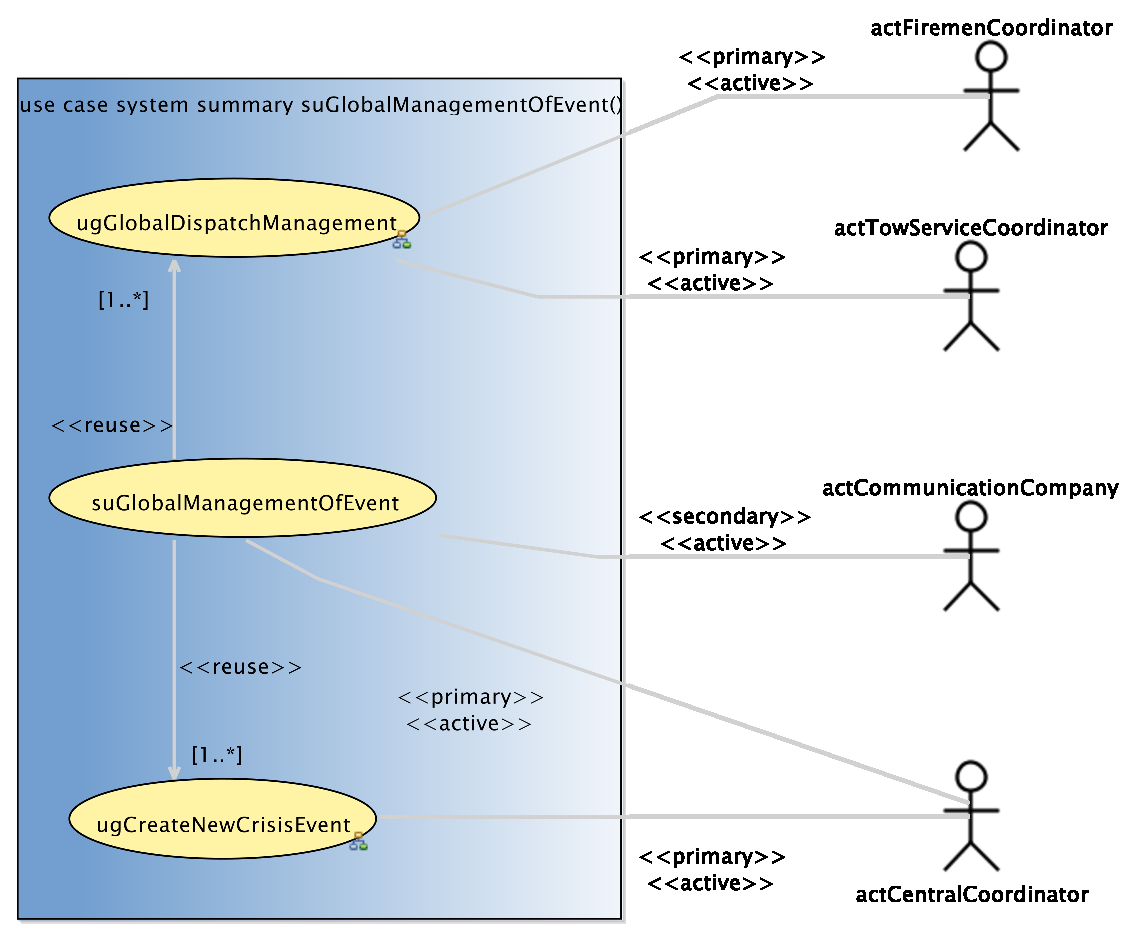
\includegraphics[
angle=0
]{./images-report-gen/usecase-model/summary/uc-suGlobalManagementOfEvent.eps}
\end{center}
\caption[lu.uni.lassy.excalibur.group09.spec Use Case Diagram: uc-suGlobalManagementOfEvent]{}
\label{fig:lu.uni.lassy.excalibur.group09.spec-RE-UCD-uc-suGlobalManagementOfEvent}
\end{figure}
\vspace{0.5cm}



%% ***************************************************************
%% User-Goal Use Cases
\subsubsection{usergoal-ugCreateNewCrisisEvent}

\label{RE-use-case-ugCreateNewCrisisEvent}


Shows the ugCreateNewCrisisEvent use-case and its actors.		  


\begin{usecase}
  \addheading{Use-Case Description}
  \addsingletwocolumnrow{Name}{ugCreateNewCrisisEvent}
  \addsingletwocolumnrow{Scope}{system}
  \addsingletwocolumnrow{Level}{usergoal}
  

\addrowheading{Primary actor(s)}
\addnumberedsinglerow{}{\msrcode{actCentralCoordinator[active]}}


\addrowheading{Secondary actor(s)}
\addnumberedsinglerow{}{\msrcode{actCommunicationCompany[active]}}
\addnumberedsinglerow{}{\msrcode{actFiremenCoordinator[passive]}}
\addnumberedsinglerow{}{\msrcode{actTowServiceCoordinator[passive]}}

\addrowheading{Goal(s) description}
\addsinglerow{Shows the ugCreateNewCrisisEvent use-case and its actors.}

\addrowheading{Reuse}
\addnumberedsinglerow{}{\msrucname{oeInitialiseNewCrisisEvent [1..*]}}
\addnumberedsinglerow{}{\msrucname{oeRequestCrisisEventLocation [0..*]}}
\addnumberedsinglerow{}{\msrucname{oeReceiveCrisisEventLocation [0..*]}}
\addnumberedsinglerow{}{\msrucname{oeConfirmCrisisEventLocation [1..*]}}
\addnumberedsinglerow{}{\msrucname{oeCreateNewCrisisEvent [1..*]}}

\addrowheading{Protocol condition(s)}
\addnumberedsinglerow{}{
none.}

\addrowheading{Pre-condition(s)}
\addnumberedsinglerow{}{
none.}

\addrowheading{Main post-condition(s)}
\addnumberedsinglerow{}{
a dispatch order including the crisis event's information such as the id, map with pins, witness's phone number, etc. is sent to nearest, free Firemen Team and Tow Service Team.}

\addrowheading{Main Steps}
\addalphanumberedsinglerow{}{the actor \msrcode{actCentralCoordinator} executes the \msrucname{oeInitialiseNewCrisisEvent} use case}
\addalphanumberedsinglerow{}{the actor \msrcode{actCentralCoordinator} executes the \msrucname{oeRequestCrisisEventLocation} use case}
\addalphanumberedsinglerow{}{the actor \msrcode{actCommunicationCompany} executes the \msrucname{oeReceiveCrisisEventLocation} use case}
\addalphanumberedsinglerow{}{the actor \msrcode{actCentralCoordinator} executes the \msrucname{oeConfirmCrisisEventLocation} use case}
\addalphanumberedsinglerow{}{the actor \msrcode{actCentralCoordinator} executes the \msrucname{oeCreateNewCrisisEvent} use case}
\addrowheading{Steps Ordering Constraints}
\addnumberedsinglerow{}{if (b) then previously (a)}
\addnumberedsinglerow{}{step (c) must be executed before step (d)}

\addrowheading{Additional Information}
\addsinglerow{
none
}

\end{usecase} 


Figure \ref{fig:lu.uni.lassy.excalibur.group09.spec-RE-UCD-uc-ugCreateNewCrisisEvent}
Shows the ugCreateNewCrisisEvent use-case and its actors.

\begin{figure}[htbp]
\begin{center}

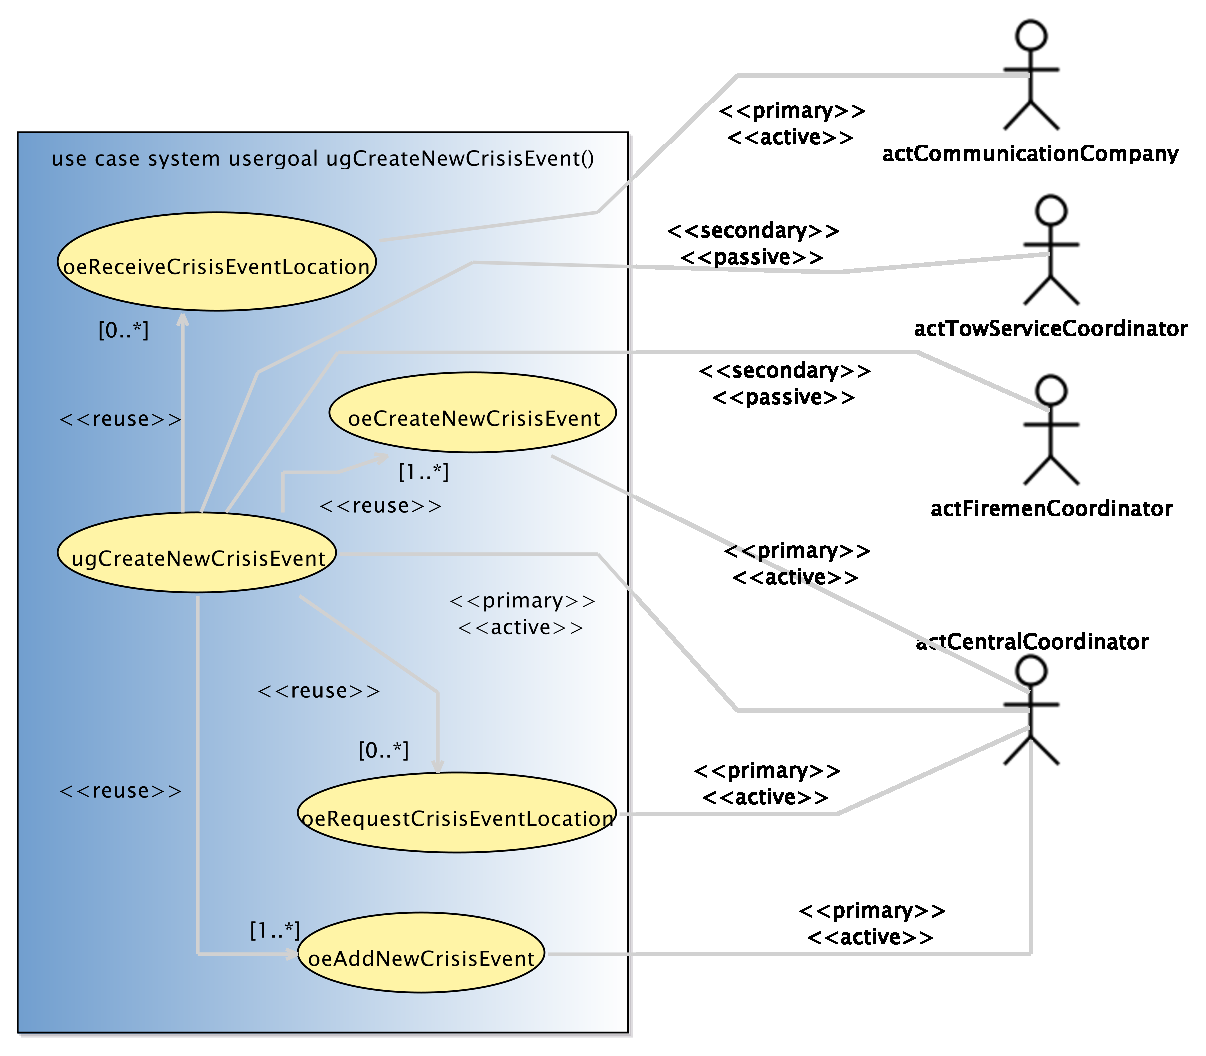
\includegraphics[
angle=0
,width=1.0\textwidth
]{./images-report-gen/usecase-model/usergoal/uc-ugCreateNewCrisisEvent.eps}
\end{center}
\caption[lu.uni.lassy.excalibur.group09.spec Use Case Diagram: uc-ugCreateNewCrisisEvent]{ugCreateNewCrisisEvent}
\label{fig:lu.uni.lassy.excalibur.group09.spec-RE-UCD-uc-ugCreateNewCrisisEvent}
\end{figure}
\vspace{0.5cm}

\subsubsection{usergoal-ugGlobalDispatchManagement}

\label{RE-use-case-ugGlobalDispatchManagement}


The goal is to have the requested coordinators arrive on the crisis event's location.		  


\begin{usecase}
  \addheading{Use-Case Description}
  \addsingletwocolumnrow{Name}{ugGlobalDispatchManagement}
  \addsingletwocolumnrow{Scope}{system}
  \addsingletwocolumnrow{Level}{usergoal}
  

\addrowheading{Primary actor(s)}
\addnumberedsinglerow{}{\msrcode{actFiremenCoordinator[active]}}
\addnumberedsinglerow{}{\msrcode{actTowServiceCoordinator[active]}}


\addrowheading{Secondary actor(s)}
\addnumberedsinglerow{}{\msrcode{actCentralCoordinator[passive]}}
\addnumberedsinglerow{}{\msrcode{actPoliceCoordinator[active]}}

\addrowheading{Goal(s) description}
\addsinglerow{The goal is to have the requested coordinators arrive on the crisis event's location.}

\addrowheading{Reuse}
\addnumberedsinglerow{}{\msrucname{oeGetCrisisEventInformation [2..*]}}
\addnumberedsinglerow{}{\msrucname{oeUpdateDispatchStatus [4..*]}}
\addnumberedsinglerow{}{\msrucname{oeRefreshMap [0..*]}}
\addnumberedsinglerow{}{\msrucname{oeMessage [0..*]}}
\addnumberedsinglerow{}{\msrucname{oeRequestHelp [0..*]}}
\addnumberedsinglerow{}{\msrucname{oeCloseCrisisEvent [2..*]}}
\addnumberedsinglerow{}{\msrucname{oeAddRequestHelp [0..*]}}

\addrowheading{Protocol condition(s)}
\addnumberedsinglerow{}{
none.}

\addrowheading{Pre-condition(s)}
\addnumberedsinglerow{}{
the sender is associated to a crisis event.}

\addrowheading{Main post-condition(s)}
\addnumberedsinglerow{}{
modifications have been made to the system and its environment concerning a crisis event.}

\addrowheading{Main Steps}
\addalphanumberedsinglerow{}{the actor \msrcode{actFiremenCoordinator} executes the \msrucname{oeGetCrisisEventInformation} use case}
\addalphanumberedsinglerow{}{the actor \msrcode{actFiremenCoordinator} executes the \msrucname{oeUpdateDispatchStatus} use case}
\addalphanumberedsinglerow{}{the actor \msrcode{actTowServiceCoordinator} executes the \msrucname{oeGetCrisisEventInformation} use case}
\addalphanumberedsinglerow{}{the actor \msrcode{actTowServiceCoordinator} executes the \msrucname{oeUpdateDispatchStatus} use case}
\addalphanumberedsinglerow{}{the actor \msrcode{actTowServiceCoordinator} executes the \msrucname{oeRefreshMap} use case}
\addalphanumberedsinglerow{}{the actor \msrcode{actTowServiceCoordinator} executes the \msrucname{oeMessage} use case}
\addalphanumberedsinglerow{}{the actor \msrcode{actFiremenCoordinator} executes the \msrucname{oeAddRequestHelp} use case}
\addalphanumberedsinglerow{}{the actor \msrcode{actFiremenCoordinator} executes the \msrucname{oeRequestHelp} use case}
\addalphanumberedsinglerow{}{the actor \msrcode{actPoliceCoordinator} executes the \msrucname{oeGetCrisisEventInformation} use case}
\addalphanumberedsinglerow{}{the actor \msrcode{actPoliceCoordinator} executes the \msrucname{oeUpdateDispatchStatus} use case}
\addalphanumberedsinglerow{}{the actor \msrcode{actFiremenCoordinator} executes the \msrucname{oeCloseCrisisEvent} use case}
\addalphanumberedsinglerow{}{the actor \msrcode{actTowServiceCoordinator} executes the \msrucname{oeCloseCrisisEvent} use case}
\addalphanumberedsinglerow{}{the actor \msrcode{actPoliceCoordinator} executes the \msrucname{oeCloseCrisisEvent} use case}
\addrowheading{Steps Ordering Constraints}
\addnumberedsinglerow{}{if step (b),(d),(j) then previously step (a),(c),(i) respectively}
\addnumberedsinglerow{}{if step (k),(l),(m) then previously step (b),(d),(j) at least two times respectively}
\addnumberedsinglerow{}{step (h) can only be executed if step (g) has at least been executed once previously}
\addnumberedsinglerow{}{if step (i) then previously step (h)}

\addrowheading{Additional Information}
\addsinglerow{
none
}

\end{usecase} 


Figure \ref{fig:lu.uni.lassy.excalibur.group09.spec-RE-UCD-uc-ugGlobalDispatchManagement}
Shows the ugGlobalDispatchManagement use-case and its actors.

\begin{figure}[htbp]
\begin{center}

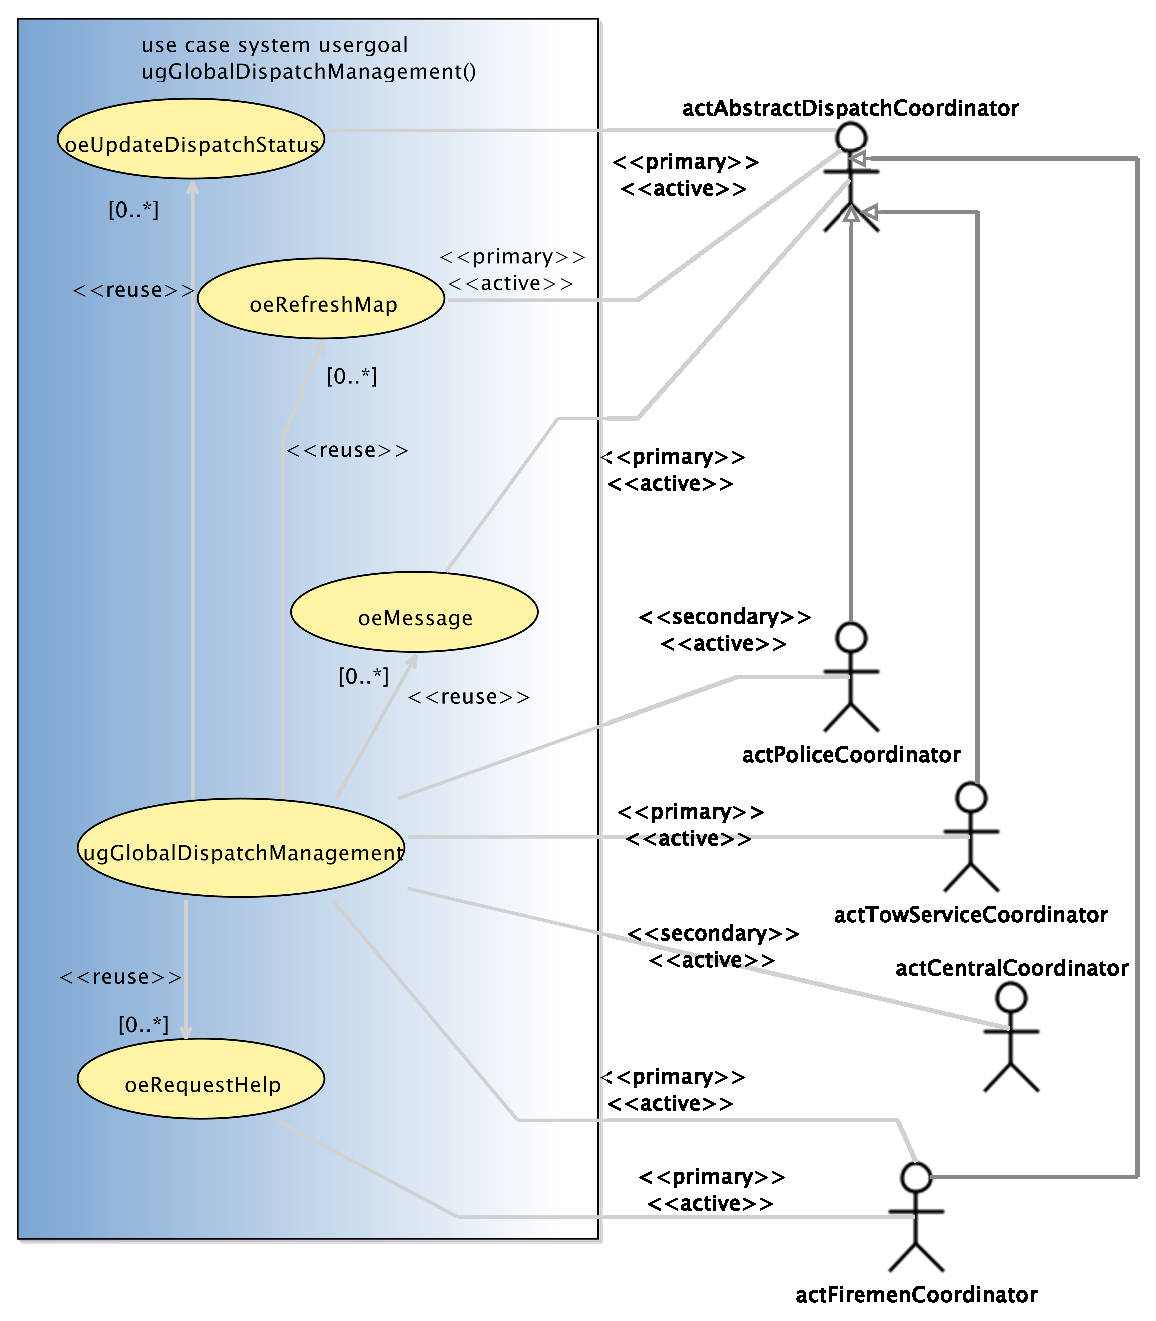
\includegraphics[
angle=0
,width=1.0\textwidth
]{./images-report-gen/usecase-model/usergoal/uc-ugGlobalDispatchManagement.eps}
\end{center}
\caption[lu.uni.lassy.excalibur.group09.spec Use Case Diagram: uc-ugGlobalDispatchManagement]{ugGlobalDispatchManagement}
\label{fig:lu.uni.lassy.excalibur.group09.spec-RE-UCD-uc-ugGlobalDispatchManagement}
\end{figure}
\vspace{0.5cm}



%% ***************************************************************
%% Subfunction Use Cases
\subsubsection{subfunction-oeConfirmCrisisEventLocation}

\label{RE-use-case-oeConfirmCrisisEventLocation}


sent to confirm the crisis event's location.		  


\begin{usecase}
  \addheading{Use-Case Description}
  \addsingletwocolumnrow{Name}{oeConfirmCrisisEventLocation}
  \addsingletwocolumnrow{Scope}{system}
  \addsingletwocolumnrow{Level}{subfunction}
  

\addrowheading{Primary actor(s)}
\addnumberedsinglerow{}{\msrcode{actCentralCoordinator[active]}}



\addrowheading{Goal(s) description}
\addsinglerow{sent to confirm the crisis event's location.}

\addrowheading{Protocol condition(s)}
\addnumberedsinglerow{}{
}

\addrowheading{Pre-condition(s)}
\addnumberedsinglerow{}{
}

\addrowheading{Main post-condition(s)}
\addnumberedsinglerow{}{
}

\addrowheading{Additional Information}
\addsinglerow{
none
}

\end{usecase} 


\subsubsection{subfunction-oeCreateNewCrisisEvent}

\label{RE-use-case-oeCreateNewCrisisEvent}


sent to create a new crisis event and to alert the corresponding coordinators.		  


\begin{usecase}
  \addheading{Use-Case Description}
  \addsingletwocolumnrow{Name}{oeCreateNewCrisisEvent}
  \addsingletwocolumnrow{Scope}{system}
  \addsingletwocolumnrow{Level}{subfunction}
  
\addrowheading{Parameters}
\addnumberedsinglerow{AdtName: ptString}{used to initialise the name field.}
\addnumberedsinglerow{AetHumanType: etHumanType}{used to initialise the type field.}
\addnumberedsinglerow{AdtPhoneNumber: dtPhoneNumber}{used to initialise the phone number field.}
\addnumberedsinglerow{AdtMapWithPin: dtMapWithPin}{used to initialise the map with pins field.}

\addrowheading{Primary actor(s)}
\addnumberedsinglerow{}{\msrcode{actCentralCoordinator[active]}}


\addrowheading{Secondary actor(s)}
\addnumberedsinglerow{}{\msrcode{actAbstractDispatchCoordinator[passive]}}

\addrowheading{Goal(s) description}
\addsinglerow{sent to create a new crisis event and to alert the corresponding coordinators.}

\addrowheading{Protocol condition(s)}
\addnumberedsinglerow{}{
none.}

\addrowheading{Pre-condition(s)}
\addnumberedsinglerow{}{
the boolean \msrcode{isLocationConfirmed} of this crisis event is set to true.}

\addrowheading{Main post-condition(s)}
\addnumberedsinglerow{}{
a dispatch order including the crisis event's information such as the id, map with pins, witness's phone number, etc. is sent to nearest, free Firemen Team and Tow Service Team.}

\addrowheading{Additional Information}
\addsinglerow{
none
}

\end{usecase} 


\subsubsection{subfunction-oeInitialiseNewCrisisEvent}

\label{RE-use-case-oeInitialiseNewCrisisEvent}


sent at the beginning of \msrcode{ugCreateNewCrisisEvent} to initialise a new crisis event.		  


\begin{usecase}
  \addheading{Use-Case Description}
  \addsingletwocolumnrow{Name}{oeInitialiseNewCrisisEvent}
  \addsingletwocolumnrow{Scope}{system}
  \addsingletwocolumnrow{Level}{subfunction}
  

\addrowheading{Primary actor(s)}
\addnumberedsinglerow{}{\msrcode{actCentralCoordinator[active]}}



\addrowheading{Goal(s) description}
\addsinglerow{sent at the beginning of \msrcode{ugCreateNewCrisisEvent} to initialise a new crisis event.}

\addrowheading{Protocol condition(s)}
\addnumberedsinglerow{}{
none.}

\addrowheading{Pre-condition(s)}
\addnumberedsinglerow{}{
none.}

\addrowheading{Main post-condition(s)}
\addnumberedsinglerow{}{
a new crisis event including an unique crisis id has been stored in the system's state.}

\addrowheading{Additional Information}
\addsinglerow{
none
}

\end{usecase} 


\subsubsection{subfunction-oeMessage}

\label{RE-use-case-oeMessage}


sent to transmit a message, comment.		  


\begin{usecase}
  \addheading{Use-Case Description}
  \addsingletwocolumnrow{Name}{oeMessage}
  \addsingletwocolumnrow{Scope}{system}
  \addsingletwocolumnrow{Level}{subfunction}
  
\addrowheading{Parameters}
\addnumberedsinglerow{AdtComment: dtComment}{}

\addrowheading{Primary actor(s)}
\addnumberedsinglerow{}{\msrcode{actAbstractDispatchCoordinator[active]}}


\addrowheading{Secondary actor(s)}
\addnumberedsinglerow{}{\msrcode{actCentralCoordinator[passive]}}
\addnumberedsinglerow{}{\msrcode{actAbstractDispatchCoordinator[multiple]}}

\addrowheading{Goal(s) description}
\addsinglerow{sent to transmit a message, comment.}

\addrowheading{Protocol condition(s)}
\addnumberedsinglerow{}{
none.}

\addrowheading{Pre-condition(s)}
\addnumberedsinglerow{}{
the sender is associated to a crisis event.}

\addrowheading{Main post-condition(s)}
\addnumberedsinglerow{}{
none.}

\addrowheading{Additional Information}
\addsinglerow{
none
}

\end{usecase} 


\subsubsection{subfunction-oeReceiveCrisisEventLocation}

\label{RE-use-case-oeReceiveCrisisEventLocation}


sent to return a map with pin.		  


\begin{usecase}
  \addheading{Use-Case Description}
  \addsingletwocolumnrow{Name}{oeReceiveCrisisEventLocation}
  \addsingletwocolumnrow{Scope}{system}
  \addsingletwocolumnrow{Level}{subfunction}
  
\addrowheading{Parameters}
\addnumberedsinglerow{AdtGeoPos: dtGeoPos}{used to initialise the first generation of the map with pins.}

\addrowheading{Primary actor(s)}
\addnumberedsinglerow{}{\msrcode{actCommunicationCompany[active]}}


\addrowheading{Secondary actor(s)}
\addnumberedsinglerow{}{\msrcode{actCentralCoordinator[passive]}}

\addrowheading{Goal(s) description}
\addsinglerow{sent to return a map with pin.}

\addrowheading{Protocol condition(s)}
\addnumberedsinglerow{}{
the geographical position must exist in google maps.}

\addrowheading{Pre-condition(s)}
\addnumberedsinglerow{}{
none.}

\addrowheading{Main post-condition(s)}
\addnumberedsinglerow{}{
an image that is the map including the pins must be returned correctly.}

\addrowheading{Additional Information}
\addsinglerow{
none
}

\end{usecase} 


\subsubsection{subfunction-oeRefreshMap}

\label{RE-use-case-oeRefreshMap}


sent to refresh the map.		  


\begin{usecase}
  \addheading{Use-Case Description}
  \addsingletwocolumnrow{Name}{oeRefreshMap}
  \addsingletwocolumnrow{Scope}{system}
  \addsingletwocolumnrow{Level}{subfunction}
  
\addrowheading{Parameters}
\addnumberedsinglerow{AdtGeoPos: dtGeoPos}{used to calculate the new pin location of the sender.}

\addrowheading{Primary actor(s)}
\addnumberedsinglerow{}{\msrcode{actAbstractDispatchCoordinator[active]}}



\addrowheading{Goal(s) description}
\addsinglerow{sent to refresh the map.}

\addrowheading{Protocol condition(s)}
\addnumberedsinglerow{}{
}

\addrowheading{Pre-condition(s)}
\addnumberedsinglerow{}{
the sender is associated to a crisis event.}

\addrowheading{Main post-condition(s)}
\addnumberedsinglerow{}{
an image that is the map including the pins must be returned correctly.}

\addrowheading{Additional Information}
\addsinglerow{
none
}

\end{usecase} 


\subsubsection{subfunction-oeRequestCrisisEventLocation}

\label{RE-use-case-oeRequestCrisisEventLocation}


sent to request a crisis event's location.		  


\begin{usecase}
  \addheading{Use-Case Description}
  \addsingletwocolumnrow{Name}{oeRequestCrisisEventLocation}
  \addsingletwocolumnrow{Scope}{system}
  \addsingletwocolumnrow{Level}{subfunction}
  
\addrowheading{Parameters}
\addnumberedsinglerow{AdtPhoneNumber: dtPhoneNumber}{}

\addrowheading{Primary actor(s)}
\addnumberedsinglerow{}{\msrcode{actCentralCoordinator[active]}}


\addrowheading{Secondary actor(s)}
\addnumberedsinglerow{}{\msrcode{actCommunicationCompany[passive]}}

\addrowheading{Goal(s) description}
\addsinglerow{sent to request a crisis event's location.}

\addrowheading{Protocol condition(s)}
\addnumberedsinglerow{}{
}

\addrowheading{Pre-condition(s)}
\addnumberedsinglerow{}{
}

\addrowheading{Main post-condition(s)}
\addnumberedsinglerow{}{
}

\addrowheading{Additional Information}
\addsinglerow{
none
}

\end{usecase} 


\subsubsection{subfunction-oeRequestHelp}

\label{RE-use-case-oeRequestHelp}


sent to request help from the corresponding team type.		  


\begin{usecase}
  \addheading{Use-Case Description}
  \addsingletwocolumnrow{Name}{oeRequestHelp}
  \addsingletwocolumnrow{Scope}{system}
  \addsingletwocolumnrow{Level}{subfunction}
  
\addrowheading{Parameters}
\addnumberedsinglerow{AetTeamType: etTeamType}{}
\addnumberedsinglerow{RequestedNumber: ptInteger}{}

\addrowheading{Primary actor(s)}
\addnumberedsinglerow{}{\msrcode{actFiremenCoordinator[active]}}


\addrowheading{Secondary actor(s)}
\addnumberedsinglerow{}{\msrcode{actAbstractDispatchCoordinator[passive]}}

\addrowheading{Goal(s) description}
\addsinglerow{sent to request help from the corresponding team type.}

\addrowheading{Protocol condition(s)}
\addnumberedsinglerow{}{
the requested number of at least one team type is greater than 0.}

\addrowheading{Pre-condition(s)}
\addnumberedsinglerow{}{
the sender is associated to a crisis event.}

\addrowheading{Main post-condition(s)}
\addnumberedsinglerow{}{
a dispatch order including the crisis event's information such as the id, map with pins, witness's phone number, etc. is sent to nearest, free requested team(s).}

\addrowheading{Additional Information}
\addsinglerow{
none
}

\end{usecase} 


\subsubsection{subfunction-oeUpdateDispatchStatus}

\label{RE-use-case-oeUpdateDispatchStatus}


sent to update the dispatch status.		  


\begin{usecase}
  \addheading{Use-Case Description}
  \addsingletwocolumnrow{Name}{oeUpdateDispatchStatus}
  \addsingletwocolumnrow{Scope}{system}
  \addsingletwocolumnrow{Level}{subfunction}
  
\addrowheading{Parameters}
\addnumberedsinglerow{AetDispatchStatus: etDispatchStatus}{}

\addrowheading{Primary actor(s)}
\addnumberedsinglerow{}{\msrcode{actAbstractDispatchCoordinator[active]}}



\addrowheading{Goal(s) description}
\addsinglerow{sent to update the dispatch status.}

\addrowheading{Protocol condition(s)}
\addnumberedsinglerow{}{
}

\addrowheading{Pre-condition(s)}
\addnumberedsinglerow{}{
}

\addrowheading{Main post-condition(s)}
\addnumberedsinglerow{}{
}

\addrowheading{Additional Information}
\addsinglerow{
none
}

\end{usecase} 





%% ***************************************************************
%% Use Case Instances
\pagebreak
\subsection{Use Case Instance(s)}


%% ***************************************************************
%% Summary Use Case Instances

	\subsubsection{Use-Case Instance - ucisuGlobalManagementOfEvent:suGlobalManagementOfEvent}
	
	Shows the suGlobaManagementOfEvent instance.		  
	\begin{operationmodel}
	\addheading{summary Use-Case Instance}
	\adddoublerow{Instantiated Use Case}{suGlobalManagementOfEvent}
	\adddoublerow{Instance ID}{ucisuGlobalManagementOfEvent}
	
	\end{operationmodel} 

	
	Figure \ref{fig:lu.uni.lassy.excalibur.group09.spec-RE-UC-uci-ucisuGlobalManagementOfEvent}
	Shows the suGlobaManagementOfEvent instance.
	
	\begin{figure}[htbp]
	\begin{center}
	
	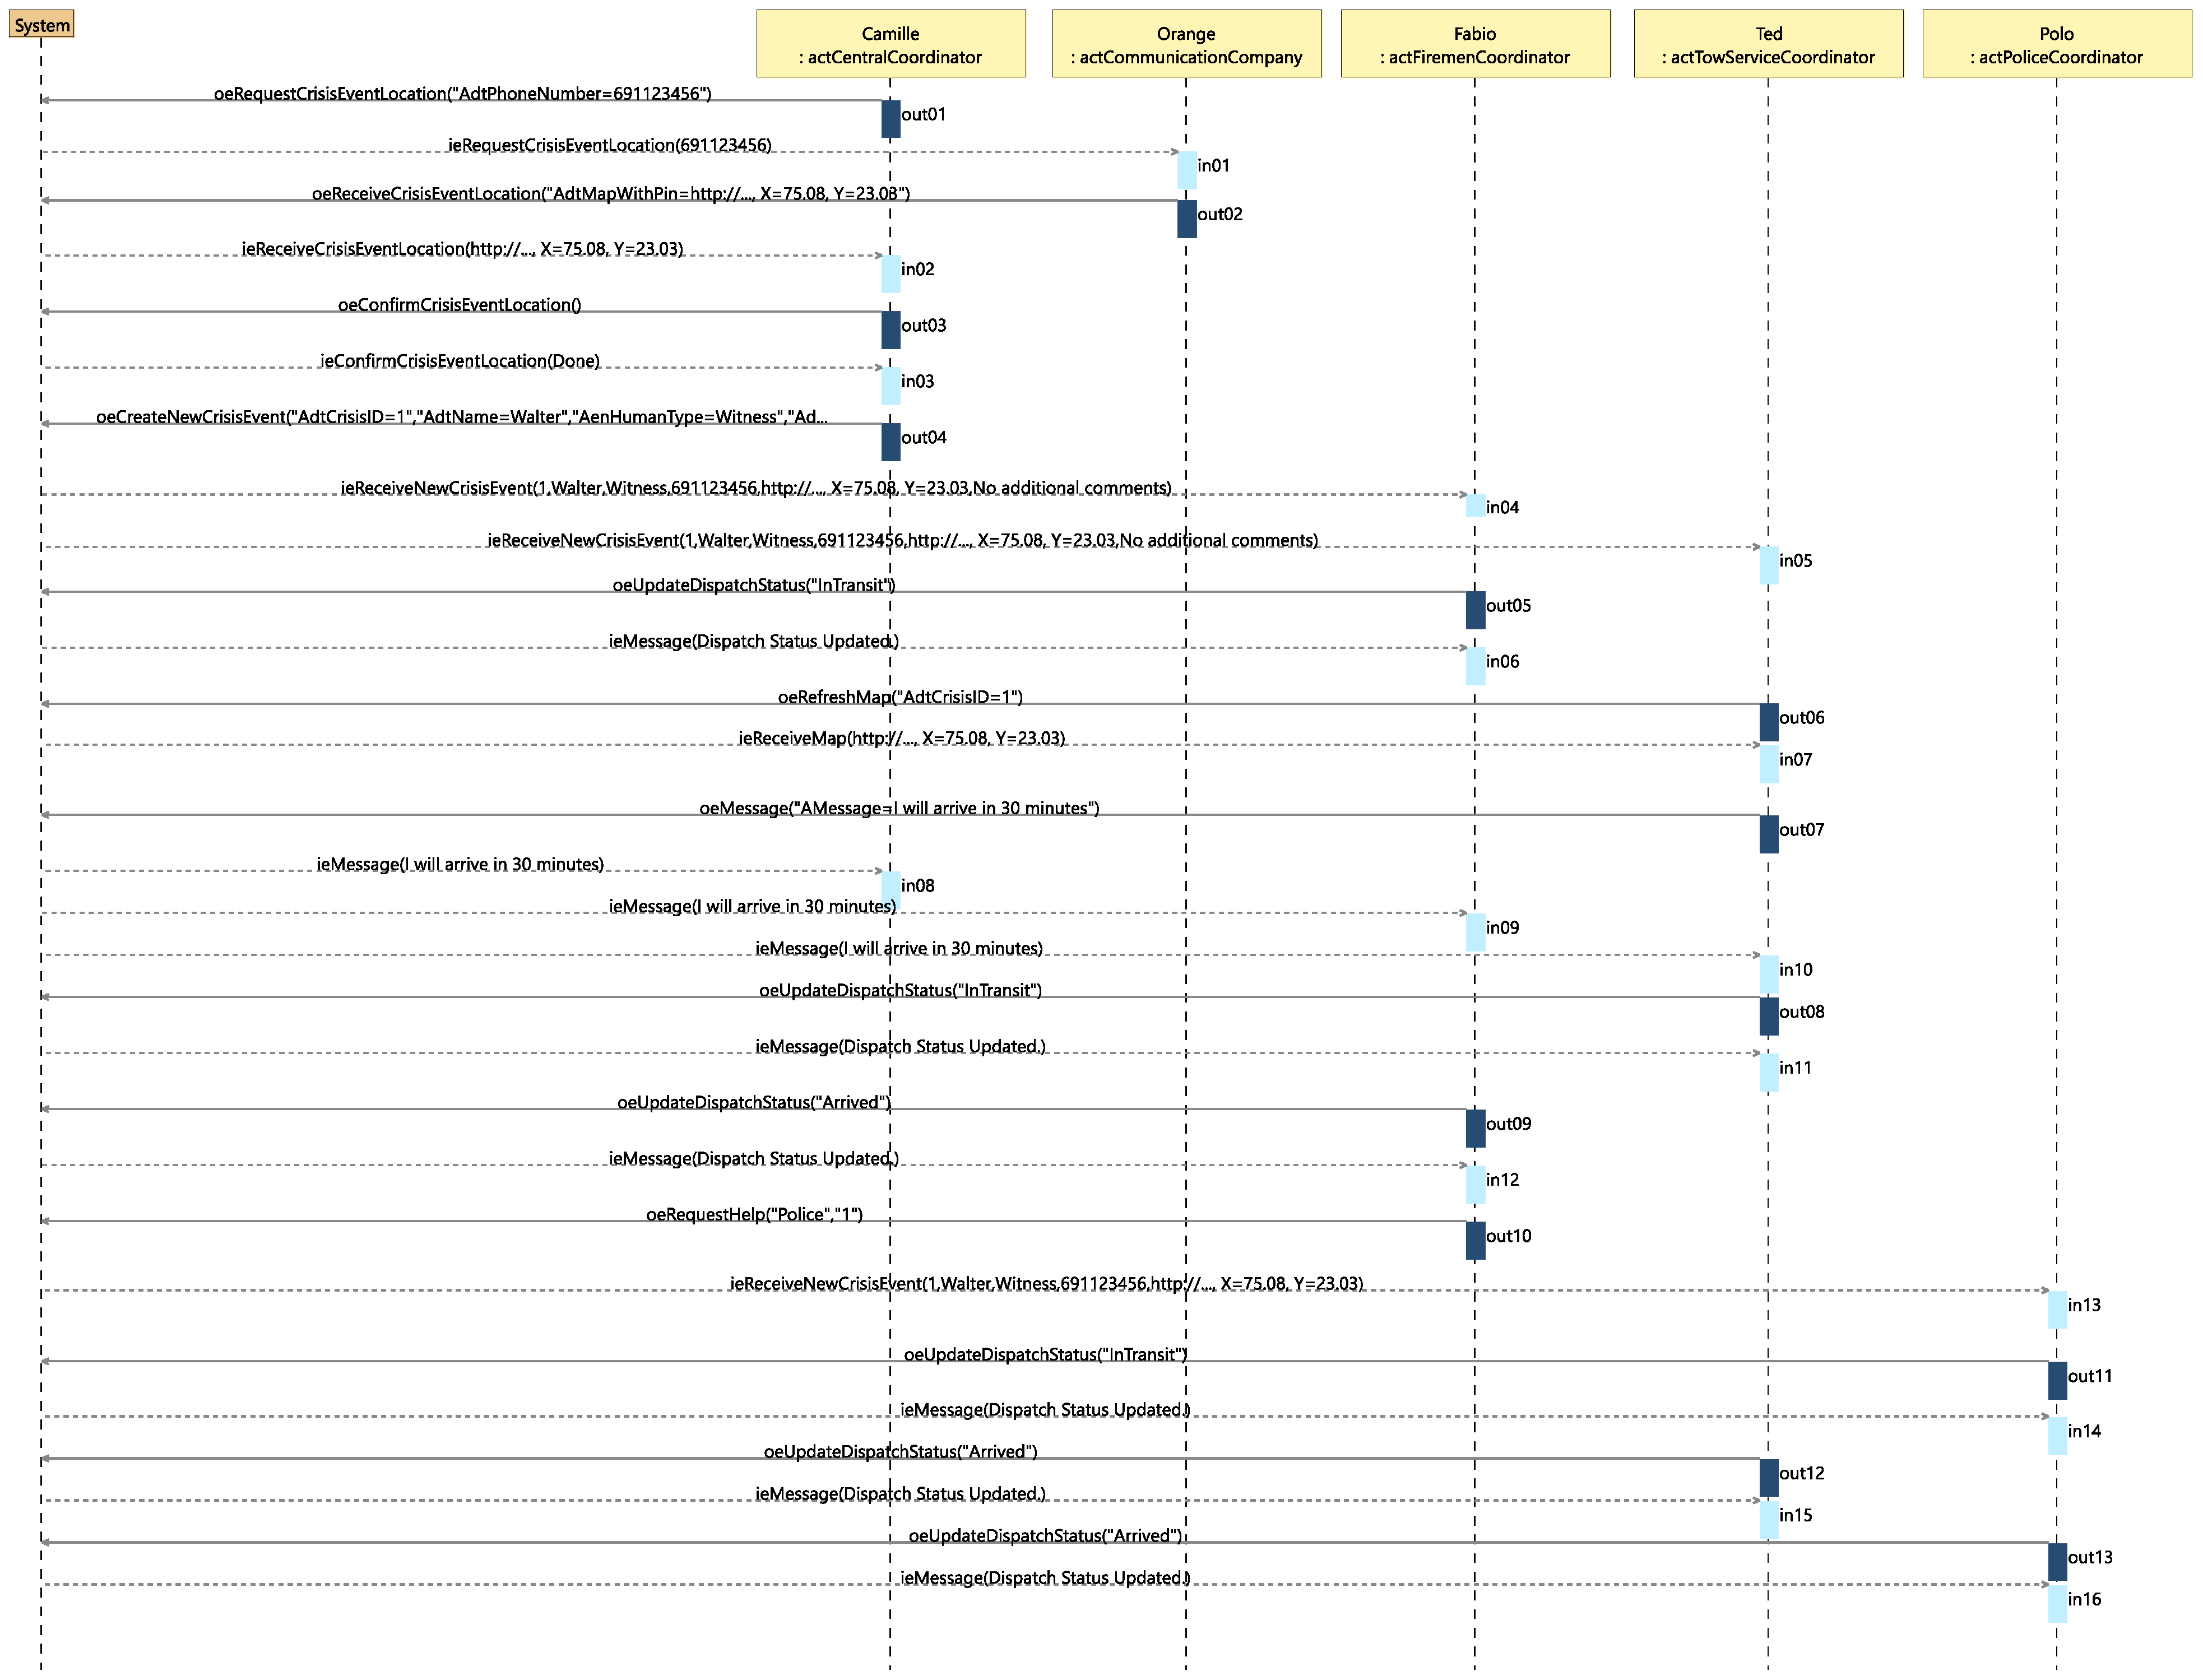
\includegraphics[
	angle=0
	]{./images-report-gen/usecase-model/summary/uci-ucisuGlobalManagementOfEvent.eps}
	\end{center}
	\caption[lu.uni.lassy.excalibur.group09.spec Sequence Diagram: uci-ucisuGlobalManagementOfEvent]{}
	\label{fig:lu.uni.lassy.excalibur.group09.spec-RE-UC-uci-ucisuGlobalManagementOfEvent}
	\end{figure}
	\vspace{0.5cm}




%% ***************************************************************
%% User-Goal Use Case Instances

	\subsubsection{Use-Case Instance - uciugCreateNewCrisiEvent:ugCreateNewCrisisEvent}
	
	Shows the ugCreateNewCrisisEvent instance.		  
	\begin{operationmodel}
	\addheading{usergoal Use-Case Instance}
	\adddoublerow{Instantiated Use Case}{ugCreateNewCrisisEvent}
	\adddoublerow{Instance ID}{uciugCreateNewCrisiEvent}
	
	\end{operationmodel} 

	
	Figure \ref{fig:lu.uni.lassy.excalibur.group09.spec-RE-UC-uci-uciugCreateNewCrisiEvent}
	Shows the ugCreateNewCrisisEvent instance.
	
	\begin{figure}[htbp]
	\begin{center}
	
	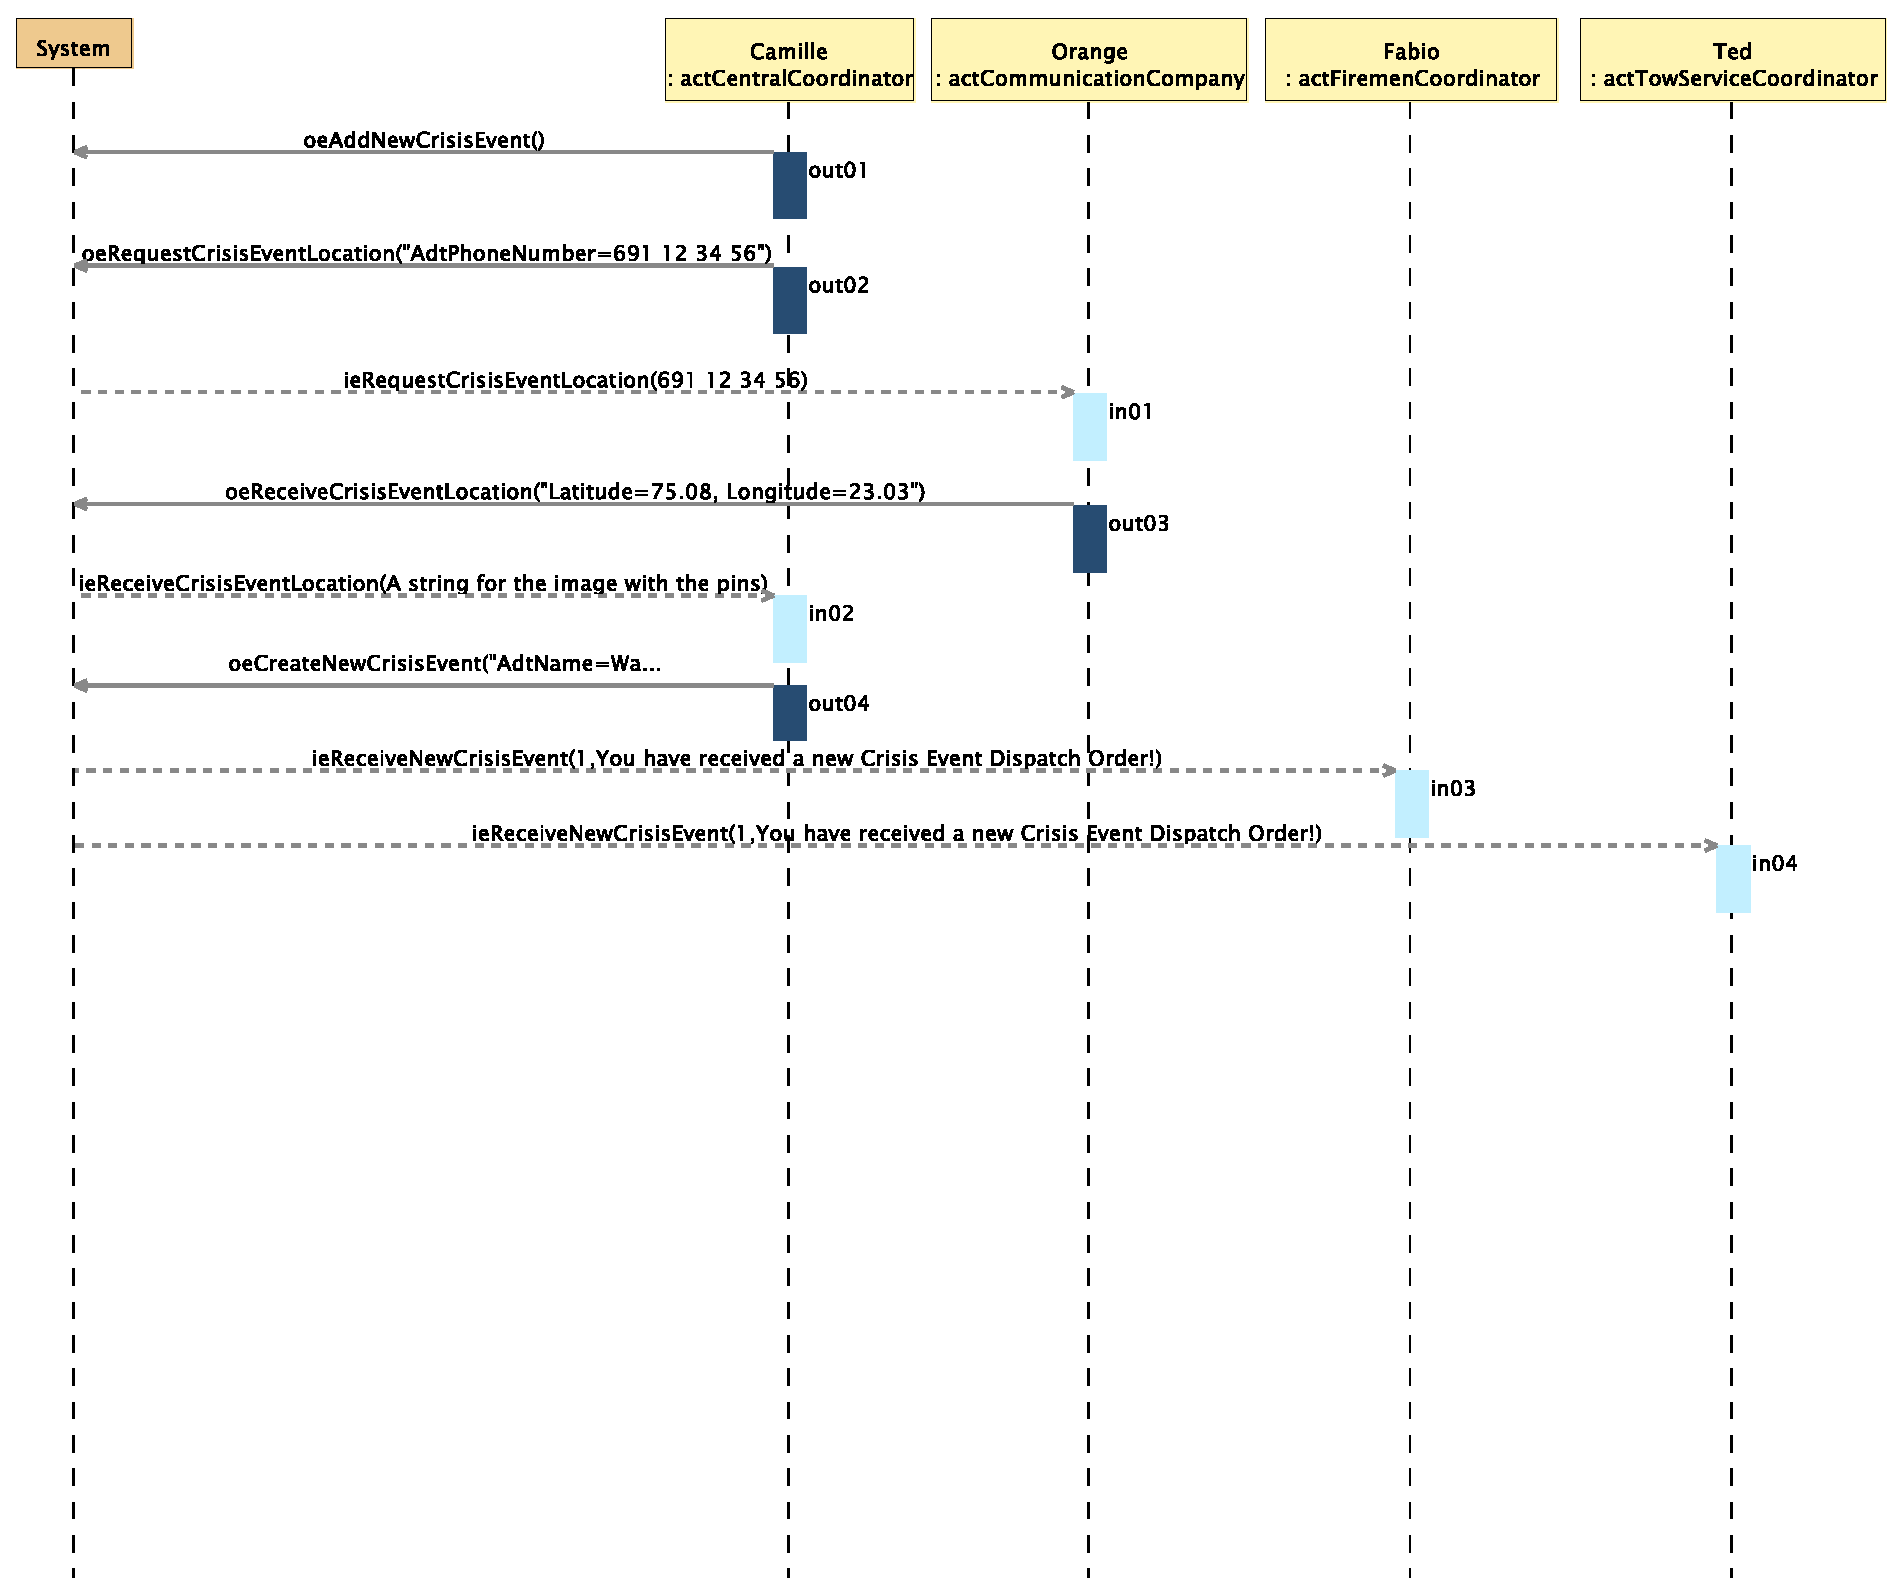
\includegraphics[
	angle=0
	,width=1.0\textwidth
	]{./images-report-gen/usecase-model/usergoal/uci-uciugCreateNewCrisiEvent.eps}
	\end{center}
	\caption[lu.uni.lassy.excalibur.group09.spec Sequence Diagram: uci-uciugCreateNewCrisiEvent]{ugCreateNewCrisisEvent}
	\label{fig:lu.uni.lassy.excalibur.group09.spec-RE-UC-uci-uciugCreateNewCrisiEvent}
	\end{figure}
	\vspace{0.5cm}


	\subsubsection{Use-Case Instance - uciugGlobalDispatchManagement:ugGlobalDispatchManagement}
	
	Shows the ugGlobalDispatchManagement instance.		  
	\begin{operationmodel}
	\addheading{usergoal Use-Case Instance}
	\adddoublerow{Instantiated Use Case}{ugGlobalDispatchManagement}
	\adddoublerow{Instance ID}{uciugGlobalDispatchManagement}
	
	\end{operationmodel} 

	
	Figure \ref{fig:lu.uni.lassy.excalibur.group09.spec-RE-UC-uci-uciugGlobalDispatchManagement}
	Shows the ugGlobalDispatchManagement instance.
	
	\begin{figure}[htbp]
	\begin{center}
	
	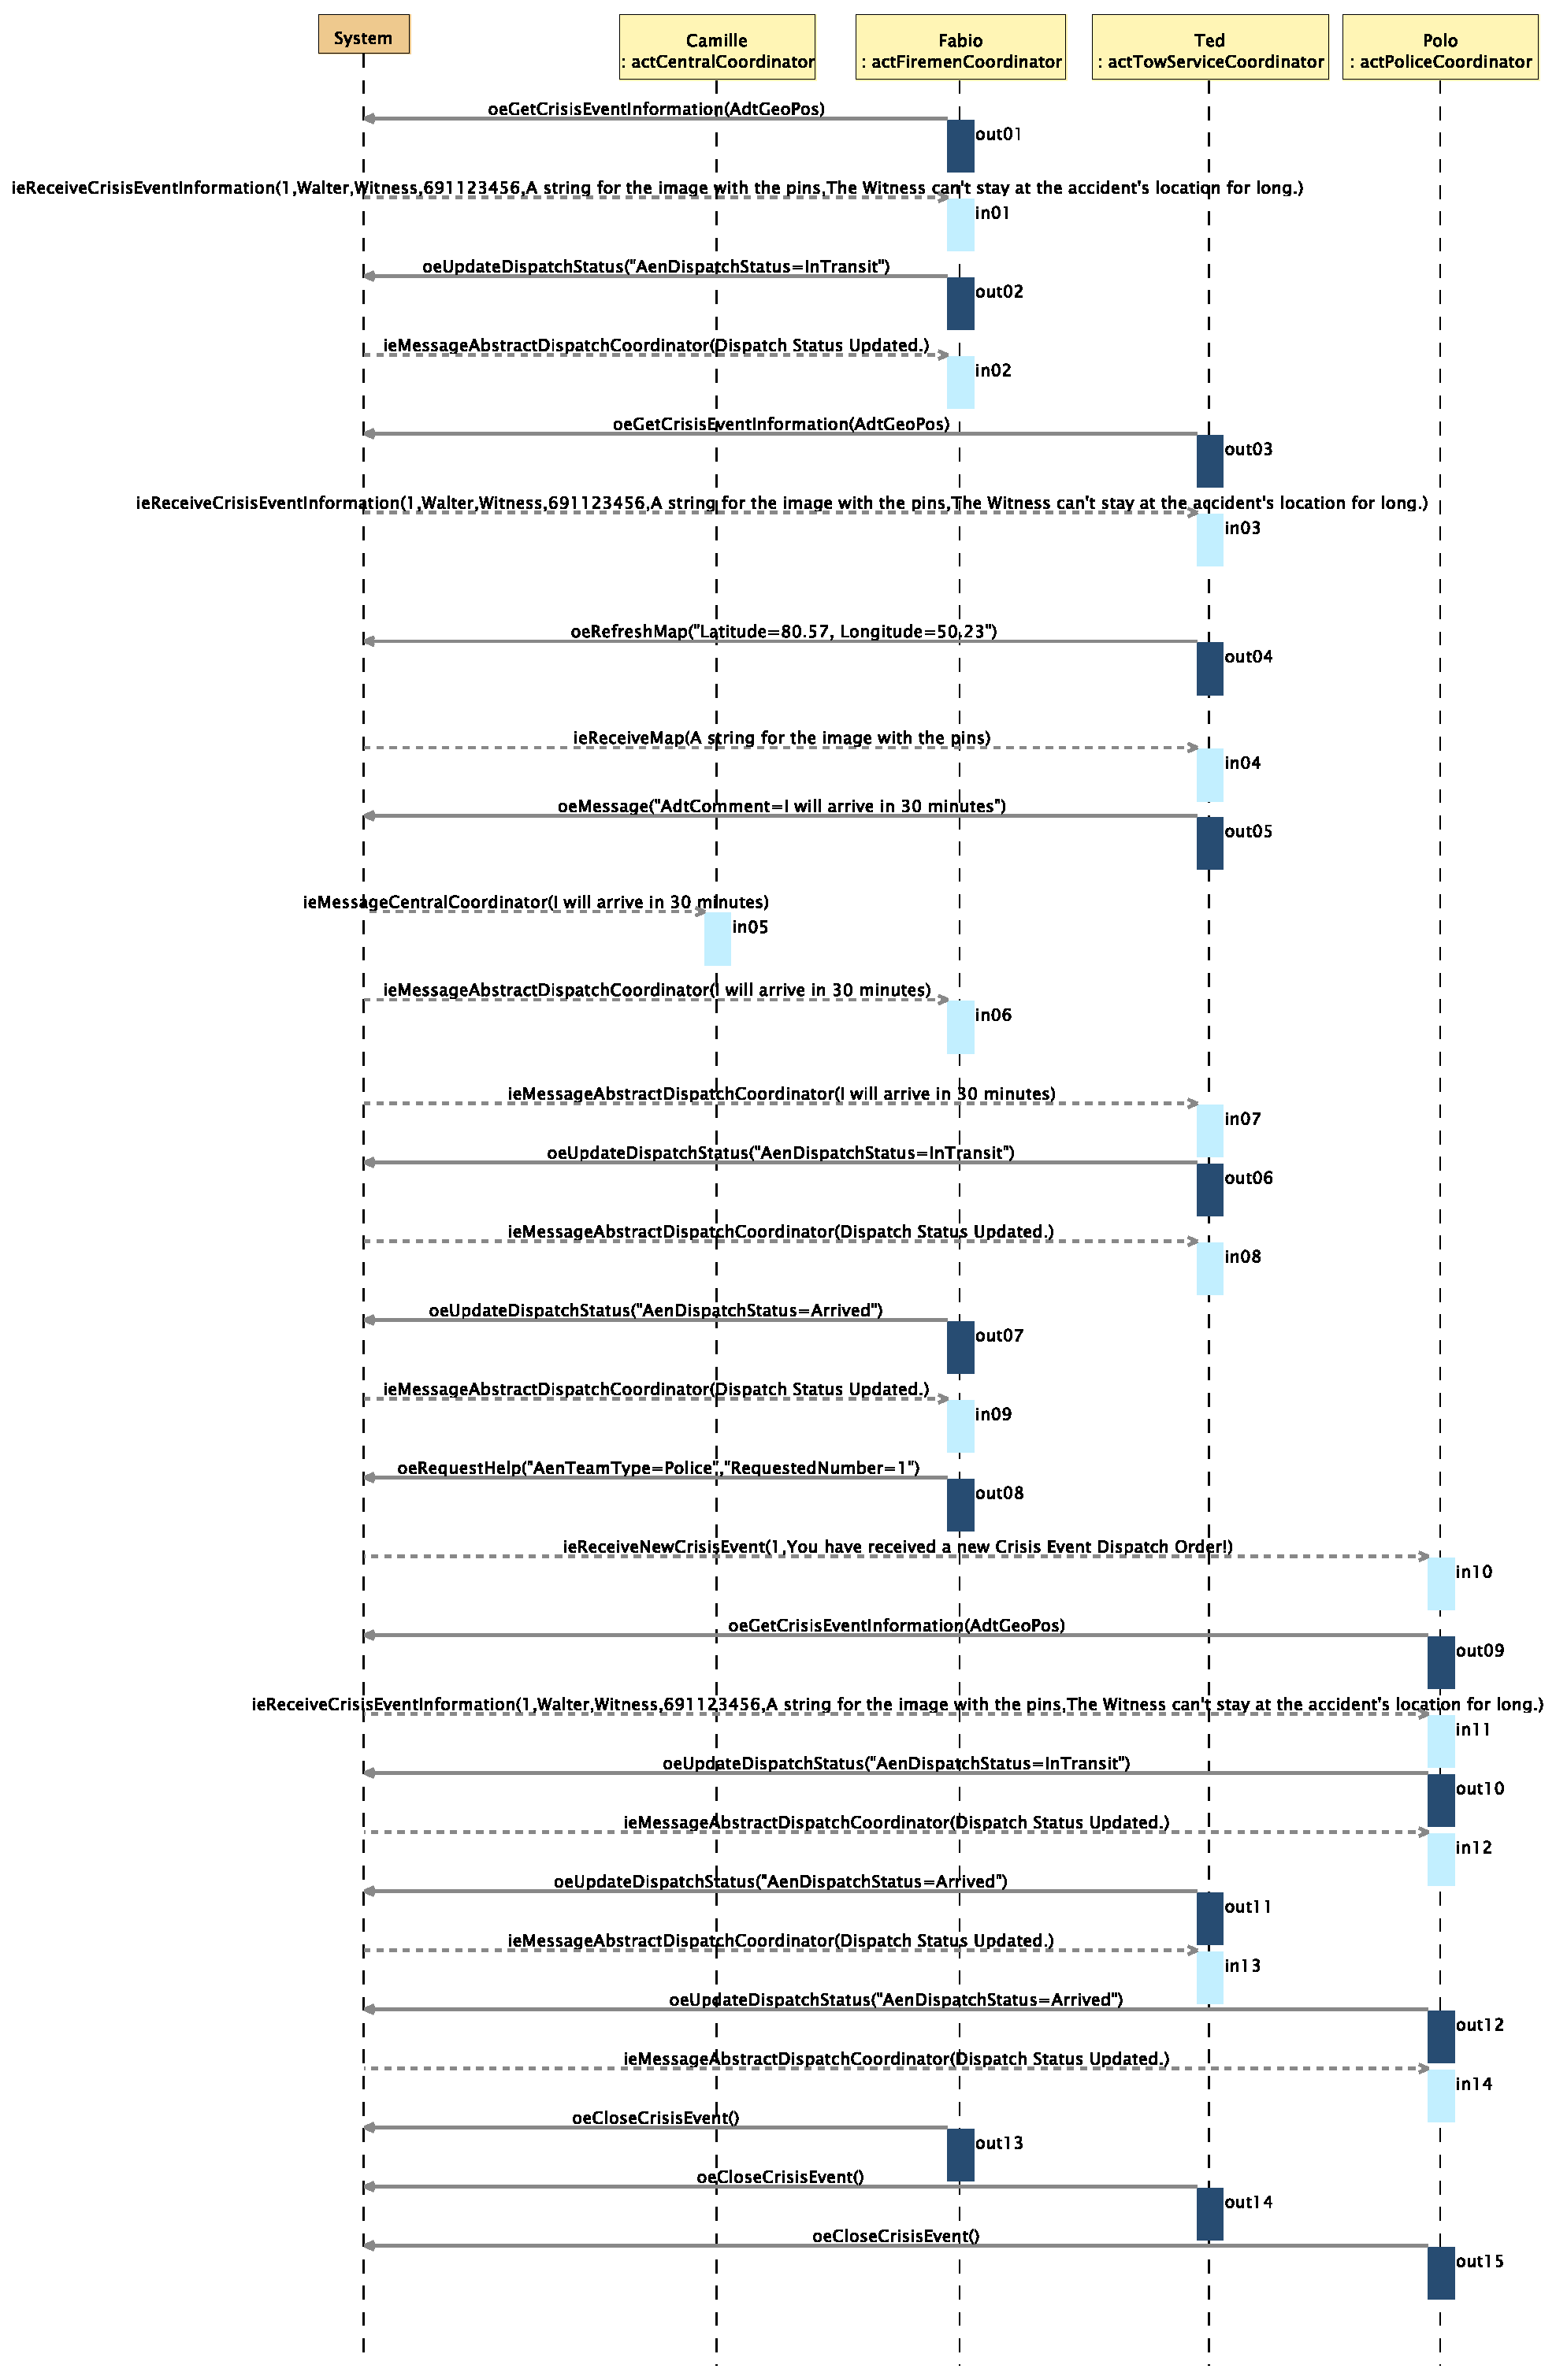
\includegraphics[
	angle=0
	,scale=0.50
	]{./images-report-gen/usecase-model/usergoal/uci-uciugGlobalDispatchManagement.eps}
	\end{center}
	\caption[lu.uni.lassy.excalibur.group09.spec Sequence Diagram: uci-uciugGlobalDispatchManagement]{ugGlobalDispatchManagement}
	\label{fig:lu.uni.lassy.excalibur.group09.spec-RE-UC-uci-uciugGlobalDispatchManagement}
	\end{figure}
	\vspace{0.5cm}




%% ***************************************************************
%% Subfunction Use Case Instances


\chapter{Environment Model}
\label{chap:lu.uni.lassy.excalibur.group09.spec-EM}


\section{Environment model view(s)}		
There are no view(s) for the \msrmessir environment model.



\section{Actors and Interfaces Descriptions}
\label{sec:lu.uni.lassy.excalibur.group09.spec-EM-Actors-Descriptions}

There are no elements in this category in the system analysed.




\chapter{Concept Model}
\label{chap:lu.uni.lassy.excalibur.group09.spec-CM}


\section{PrimaryTypes-Classes}
\subsection{Local view 12}
\label{sec:lu.uni.lassy.excalibur.group09.spec-CM-view-local-PrimaryTypes-Classes-12}
Figure \ref{fig:lu.uni.lassy.excalibur.group09.spec-CM-view-local-PrimaryTypes-Classes-12} Main view of the concept model



\begin{figure}[htbp] 
\label{fig:lu.uni.lassy.excalibur.group09.spec-CM}
\begin{center}
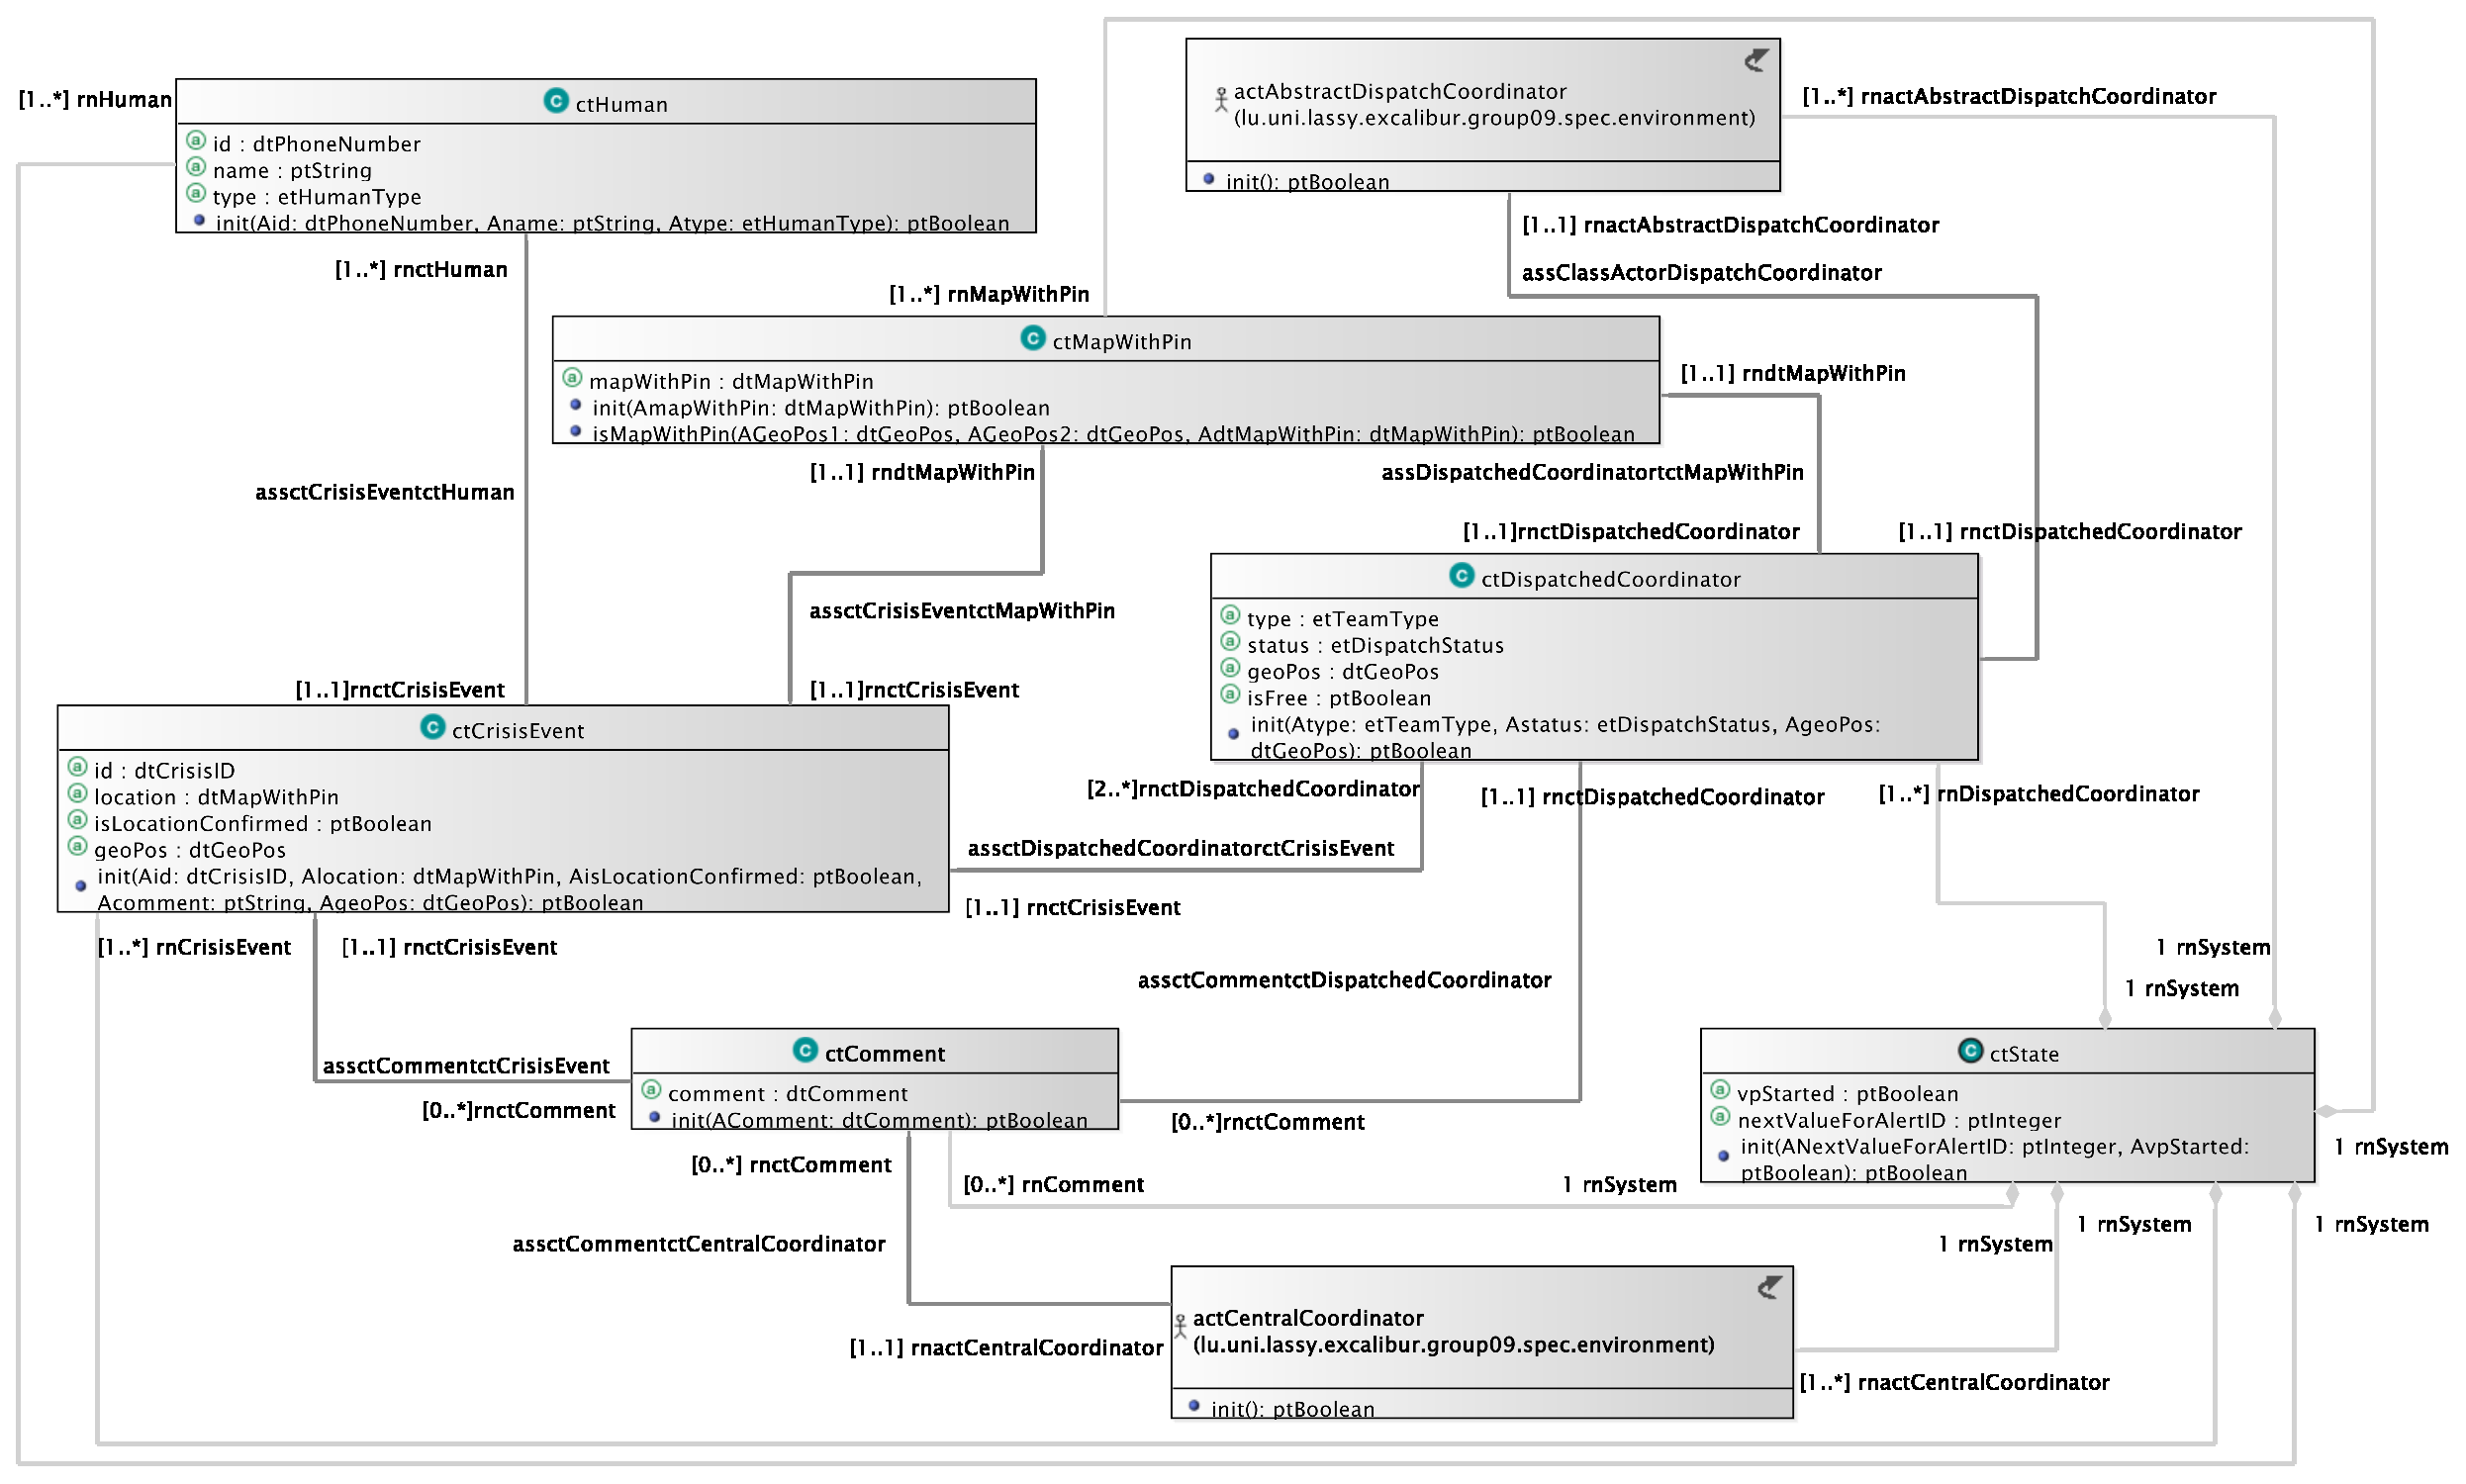
\includegraphics[
angle=90
,height=1.0\textheight
]{./images-report-gen/concept-model/local/PrimaryTypes-Classes/12/cm-ctAssociations.eps}
\end{center}
\caption[Concept Model - PrimaryTypes-Classes local view 12 - Main view of the concept model]{Concept Model - PrimaryTypes-Classes local view 12. Main view of the concept model.}
\label{fig:lu.uni.lassy.excalibur.group09.spec-CM-view-local-PrimaryTypes-Classes-12}
\end{figure}
\vspace{0.5cm} 




\section{PrimaryTypes-Datatypes}
\subsection{Local view 15}
\label{sec:lu.uni.lassy.excalibur.group09.spec-CM-view-local-PrimaryTypes-Datatypes-15}
Figure \ref{fig:lu.uni.lassy.excalibur.group09.spec-CM-view-local-PrimaryTypes-Datatypes-15} View of all the datatypes



\begin{figure}[htbp] 
\label{fig:lu.uni.lassy.excalibur.group09.spec-CM}
\begin{center}
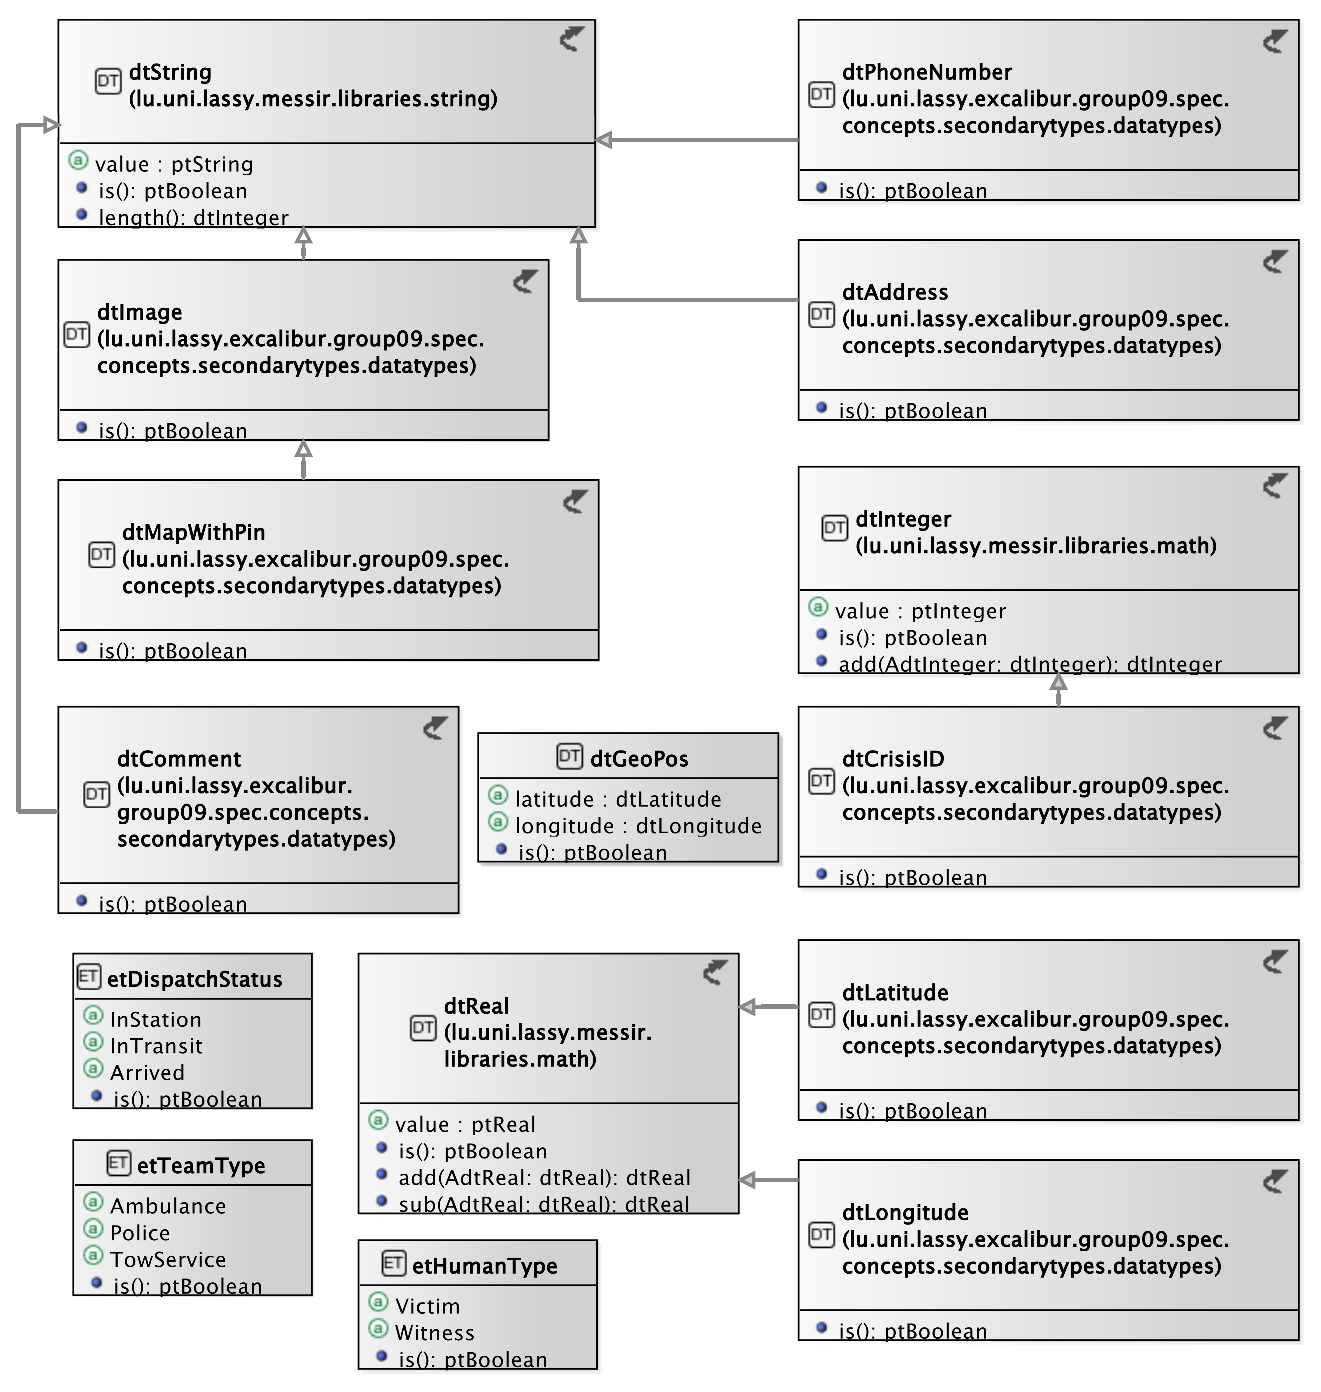
\includegraphics[
angle=0
,width=1.0\textwidth
]{./images-report-gen/concept-model/local/PrimaryTypes-Datatypes/15/cm-dt.eps}
\end{center}
\caption[Concept Model - PrimaryTypes-Datatypes local view 15 - View of all the datatypes]{Concept Model - PrimaryTypes-Datatypes local view 15. View of all the datatypes.}
\label{fig:lu.uni.lassy.excalibur.group09.spec-CM-view-local-PrimaryTypes-Datatypes-15}
\end{figure}
\vspace{0.5cm} 

\subsection{Local view 16}
\label{sec:lu.uni.lassy.excalibur.group09.spec-CM-view-local-PrimaryTypes-Datatypes-16}
Figure \ref{fig:lu.uni.lassy.excalibur.group09.spec-CM-view-local-PrimaryTypes-Datatypes-16} View of all the different modes for the coordinators/actors



\begin{figure}[htbp] 
\label{fig:lu.uni.lassy.excalibur.group09.spec-CM}
\begin{center}
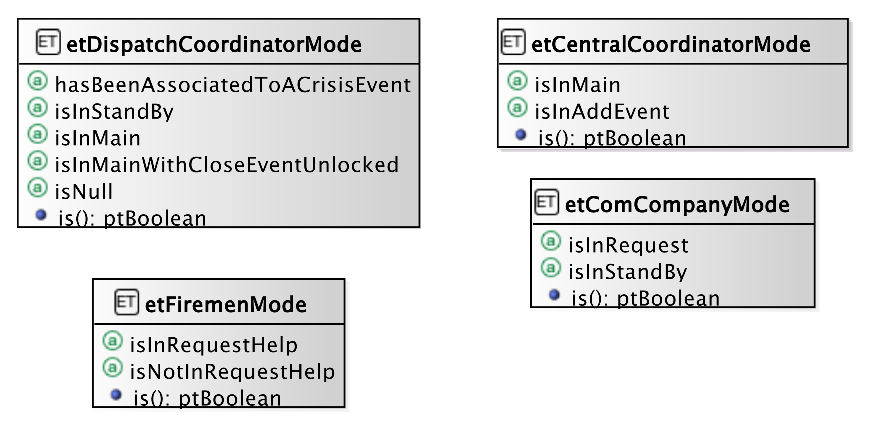
\includegraphics[
angle=0
,scale=0.80
]{./images-report-gen/concept-model/local/PrimaryTypes-Datatypes/16/cm-etModes.eps}
\end{center}
\caption[Concept Model - PrimaryTypes-Datatypes local view 16 - View of all the different modes for ]{Concept Model - PrimaryTypes-Datatypes local view 16. View of all the different modes for the coordinators/actors.}
\label{fig:lu.uni.lassy.excalibur.group09.spec-CM-view-local-PrimaryTypes-Datatypes-16}
\end{figure}
\vspace{0.5cm} 










\section{Concept Model Types Descriptions}
This section provides the textual descriptions of all the types defined in the concept model and that can be part of the graphical views provided.

\subsection{Primary types - Class types descriptions}




The table below is providing comments on the graphical views given for the class types of the primary types. Type logical operations are precisely specified in the operation model.

\begin{datadictionary}
\addheading{Classes}

\adddoublerow{ctComment}{A class containing a comment.}
\adddoubletwocolumnrow{attribute}{\msrcode{comment: dtComment}}{}
\adddoubletwocolumnrow{operation}{\msrcode{init(AComment:dtComment):ptBoolean}}{}
\adddoublerow{ctCrisisEvent}{A class containing the attributes identifying a crisis event.}
\adddoubletwocolumnrow{attribute}{\msrcode{id: dtCrisisID}}{}
\adddoubletwocolumnrow{attribute}{\msrcode{isLocationConfirmed: ptBoolean}}{}
\adddoubletwocolumnrow{attribute}{\msrcode{location: dtMapWithPin}}{}
\adddoubletwocolumnrow{operation}{\msrcode{init(Aid:dtCrisisID, Alocation:dtMapWithPin, AisLocationConfirmed:ptBoolean, Acomment:ptString, AgeoPos:dtGeoPos):ptBoolean}}{}
\adddoublerow{ctDispatchedCoordinator}{A class containing the attributes identifying a dispatched team.}
\adddoubletwocolumnrow{attribute}{\msrcode{status: etDispatchStatus}}{}
\adddoubletwocolumnrow{attribute}{\msrcode{type: etTeamType}}{}
\adddoubletwocolumnrow{operation}{\msrcode{init(Atype:etTeamType, Astatus:etDispatchStatus, AgeoPos:dtGeoPos):ptBoolean}}{}
\adddoublerow{ctHuman}{A class containing the attributes identifying an human.}
\adddoubletwocolumnrow{attribute}{\msrcode{id: dtPhoneNumber}}{}
\adddoubletwocolumnrow{attribute}{\msrcode{name: ptString}}{}
\adddoubletwocolumnrow{attribute}{\msrcode{type: etHumanType}}{}
\adddoubletwocolumnrow{operation}{\msrcode{init(Aid:dtPhoneNumber, Aname:ptString, Atype:etHumanType):ptBoolean}}{}
\adddoublerow{ctMapWithPin}{A class containing an image which is the map including the pins.}
\adddoubletwocolumnrow{attribute}{\msrcode{mapWithPin: dtMapWithPin}}{}
\adddoubletwocolumnrow{operation}{\msrcode{init(AmapWithPin:dtMapWithPin):ptBoolean}}{}
\adddoublerow{ctState}{used to model the system.}
\adddoubletwocolumnrow{attribute}{\msrcode{vpStarted: ptBoolean}}{}
\adddoubletwocolumnrow{operation}{\msrcode{init(ANextValueForAlertID:ptInteger, AvpStarted:ptBoolean):ptBoolean}}{}
\end{datadictionary}

\subsection{Primary types - Datatypes types descriptions}





The table below is providing comments on the graphical views given for the datatype types of the primary types.


\begin{datadictionary}
\addheading{Datatypes}

\adddoublerow{dtGeoPos}{Two Real numbers used to identify a geographical position on earth.}
\adddoubletwocolumnrow{attribute}{\msrcode{latitude: dtLatitude}}{}
\adddoubletwocolumnrow{attribute}{\msrcode{longitude: dtLongitude}}{}
\adddoubletwocolumnrow{operation}{\msrcode{is():ptBoolean}}{}
\end{datadictionary}


\begin{datadictionary}
\addheading{Enumerations}

\adddoublerow{etCentralCoordinatorMode}{Modes of the Central Coordinator to identify what operations he/she can do at what moment.}
\adddoubletwocolumnrow{operation}{\msrcode{is():ptBoolean}}{}
\adddoublerow{etComCompanyMode}{Modes of the Communication Company to identify what operations it can do at what moment.}
\adddoubletwocolumnrow{operation}{\msrcode{is():ptBoolean}}{}
\adddoublerow{etDispatchCoordinatorMode}{Modes of a dispatched Coordinator to identify what operations he/she can do at what moment.}
\adddoubletwocolumnrow{operation}{\msrcode{is():ptBoolean}}{}
\adddoublerow{etDispatchStatus}{A String used to identify a dispatch status.}
\adddoublerow{etFiremenMode}{Additional mode for the Firemen Coordinator to identify what operations he/she can do at what moment.}
\adddoubletwocolumnrow{operation}{\msrcode{is():ptBoolean}}{}
\adddoublerow{etHumanType}{A String used to identify an Human type.}
\adddoublerow{etTeamType}{A String used to identify a team type.}
\end{datadictionary}






\subsection{Primary types - Association types descriptions}




The table below is providing comments on the association types of the primary types.

\begin{associationtypes}
\addheading{Undirected associations}
\adddoublerow{assctCrisisEventctHuman}{Association of a crisis event to an human.}
\adddoublerow{assctDispatchedCoordinatoractAbstractDispatchCoordinator}{Association of a dispatched coordinator to an actor of the same type.}
\adddoublerow{assctDispatchedCoordinatorctCrisisEvent}{Association of a dispatched coordinator to a crisis event.}
\end{associationtypes}

\subsection{Primary types - Aggregation types descriptions}


There are no aggregation types for the primary types.


\subsubsection{Primary types - Composition types descriptions}



There are no composition types for the primary types.


\subsection{Secondary types - Class types descriptions}



There are no elements in this category in the system analysed.
		

\subsection{Secondary types - Datatypes types descriptions}





The table below is providing comments on the graphical views given for the datatype types of the secondary types.

\begin{datadictionary}
\addheading{Datatypes}

\adddoublerow{dtAddress}{A String used to identify an address.}
\addsingletwocolumnrow{extends}{dtString}
\adddoubletwocolumnrow{operation}{\msrcode{is():ptBoolean}}{}
\adddoublerow{dtCrisisID}{An Integer used to identify a crisis id.}
\addsingletwocolumnrow{extends}{dtInteger}
\adddoubletwocolumnrow{operation}{\msrcode{is():ptBoolean}}{}
\adddoublerow{dtImage}{A String used to identify an image.}
\addsingletwocolumnrow{extends}{dtString}
\adddoubletwocolumnrow{operation}{\msrcode{is():ptBoolean}}{}
\adddoublerow{dtLatitude}{used to define a latitude value of a geograpical positions on earth.}
\addsingletwocolumnrow{extends}{dtReal}
\adddoubletwocolumnrow{operation}{\msrcode{is():ptBoolean}}{}
\adddoublerow{dtLongitude}{used to define a longitude value of a geograpical positions on earth.}
\addsingletwocolumnrow{extends}{dtReal}
\adddoubletwocolumnrow{operation}{\msrcode{is():ptBoolean}}{}
\adddoublerow{dtMapWithPin}{An image which is a map including pins.}
\addsingletwocolumnrow{extends}{dtImage}
\adddoubletwocolumnrow{operation}{\msrcode{is():ptBoolean}}{}
\adddoublerow{dtPhoneNumber}{A String used to store a phone number.}
\addsingletwocolumnrow{extends}{dtString}
\adddoubletwocolumnrow{operation}{\msrcode{is():ptBoolean}}{}
\end{datadictionary}





\subsection{Secondary types - Association types descriptions}



There are no association types for the secondary types.



\subsection{Secondary types - Aggregation types descriptions}



There are no aggregation types for the secondary types.



\subsection{Secondary types - Composition types descriptions}



There are no composition types for the secondary types.





\chapter{Operation Model}
\label{chap:lu.uni.lassy.excalibur.group09.spec-OM}

This section contains the operation schemes of each operation defined in either an actor, its output interface, in a primary or secondary type (class, datatype or enumeration types). 
The \msrmessir OCL code listing is joined to the comment table.

\lstset{
float,
basicstyle=\scriptsize,
language=Messir,
breakatwhitespace=false,
tabsize=2,
breaklines=true,
numbers=left,
emptylines=1,
numbersep=5pt,
showspaces=false,
showstringspaces=false,
showtabs=false
} 


%% ***************************************************************
%% operations for: Environment-Out Interface Operation Schemes

		
\section{Environment - Out Interface Operation Scheme for actAbstractDispatchCoordinator}
\label{OM-EM-OutInterface-OS-actAbstractDispatchCoordinator}
\subsection{Operation Model for oeCloseCrisisEvent}

\label{OM-oeCloseCrisisEvent}


The \msrcode{oeCloseCrisisEvent} operation has the following properties:

	\begin{operationmodel}
	\addheading{Operation}
	\adddoublerow{oeCloseCrisisEvent}{sent to close up the associated crisis event for the current coordinator.
	 }


	\addrowheading{Return type}
	\addsinglerow{ptBoolean}

	\addrowheading{Pre-Condition (protocol)}
	\addnumberedsinglerow{PreP}{The dispatch coordinator's mode is \msrcode{isInMainWithCloseEventUnlocked}.}
		
	\addrowheading{Pre-Condition (functional)}
	\addnumberedsinglerow{PreF}{it is supposed that a dispatched coordinator can only be associated to a single crisis event at the same time.}

	\addrowheading{Post-Condition (functional)}
	\addnumberedsinglerow{PostF}{The coordinator's attribute\msrcode{isFree} is set back to true and can thus be associated to another crisis event.}

	\addrowheading{Post-Condition (protocol)}
	\addnumberedsinglerow{PostP}{The dispatch coordinator is no longer associated to the current crisis event.}
	\addnumberedsinglerow{PostP}{The dispatch coordinator's mode is set to \msrcode{isInStandBy}.}
	\end{operationmodel}



	
	
	
	






\subsection{Operation Model for oeGetCrisisEventInformation}

\label{OM-oeGetCrisisEventInformation}


The \msrcode{oeGetCrisisEventInformation} operation has the following properties:

	\begin{operationmodel}
	\addheading{Operation}
	\adddoublerow{oeGetCrisisEventInformation}{sent to get the stored information of the crisis event to which the dispatch coordinator is associated.}

	\addrowheading{Parameters}
	\addnumbereddoublerow{}{AdtGeoPos: dtGeoPos}{a geographical position that identifies the actor's current position.} 

	\addrowheading{Return type}
	\addsinglerow{ptBoolean}

	\addrowheading{Pre-Condition (protocol)}
	\addnumberedsinglerow{PreP}{The dispatch coordinator's mode has been set to \msrcode{hasBeenAssociatedToACrisisEvent}.}
		
	\addrowheading{Pre-Condition (functional)}
	\addnumberedsinglerow{PreF}{it is supposed that a dispatched coordinator can only be associated to a single crisis event at the same time.}
	\addnumberedsinglerow{PreF}{the\msrcode{GeoPos} given by the coordinator is a valid one.}

	\addrowheading{Post-Condition (functional)}
	\addnumberedsinglerow{PostF}{the map with pins returned to coordinator includes a pin of the actor's current position and another one of the crisis event's location.}

	\addrowheading{Post-Condition (protocol)}
	\addnumberedsinglerow{PostP}{The dispatch coordinator's mode has been set to \msrcode{isInMain}.}
	\end{operationmodel}



	
	
	
	






\subsection{Operation Model for oeMessage}

\label{OM-oeMessage}


The \msrcode{oeMessage} operation has the following properties:

	\begin{operationmodel}
	\addheading{Operation}
	\adddoublerow{oeMessage}{sent to transmit a message.
	 }

	\addrowheading{Parameters}
	\addnumbereddoublerow{}{AdtComment: dtComment}{} 

	\addrowheading{Return type}
	\addsinglerow{ptBoolean}

	\addrowheading{Pre-Condition (protocol)}
	\addnumberedsinglerow{PreP}{The dispatch coordinator's mode has is \msrcode{isInMain} or \msrcode{isInMainWithCloseEventUnlocked}.}
		
	\addrowheading{Pre-Condition (functional)}
	\addnumberedsinglerow{PreF}{it is supposed that a dispatched coordinator can only be associated to a single crisis event at the same time.}


	\end{operationmodel}



	
	
	
	






\subsection{Operation Model for oeRefreshMap}

\label{OM-oeRefreshMap}


The \msrcode{oeRefreshMap} operation has the following properties:

	\begin{operationmodel}
	\addheading{Operation}
	\adddoublerow{oeRefreshMap}{sent to refresh the map.}

	\addrowheading{Parameters}
	\addnumbereddoublerow{}{AdtGeoPos: dtGeoPos}{the coordinator's current geographical position.} 

	\addrowheading{Return type}
	\addsinglerow{ptBoolean}

	\addrowheading{Pre-Condition (protocol)}
	\addnumberedsinglerow{PreP}{The dispatch coordinator's is \msrcode{isInMain} or \msrcode{isInMainWithCloseEventUnlocked}.}
		
	\addrowheading{Pre-Condition (functional)}
	\addnumberedsinglerow{PreF}{it is supposed that a dispatched coordinator can only be associated to a single crisis event at the same time.}
	\addnumberedsinglerow{PreF}{the\msrcode{GeoPos} given by the coordinator is a valid one.}

	\addrowheading{Post-Condition (functional)}
	\addnumberedsinglerow{PostF}{the map with pins returned to the coordinator includes a pin of the actor's current position and another one of the crisis event's location.}

	\end{operationmodel}



	
	
	
	






\subsection{Operation Model for oeUpdateDispatchStatus}

\label{OM-oeUpdateDispatchStatus}


The \msrcode{oeUpdateDispatchStatus} operation has the following properties:

	\begin{operationmodel}
	\addheading{Operation}
	\adddoublerow{oeUpdateDispatchStatus}{sent to update the dispatch status.}

	\addrowheading{Parameters}
	\addnumbereddoublerow{}{AetDispatchStatus: etDispatchStatus}{} 

	\addrowheading{Return type}
	\addsinglerow{ptBoolean}

	\addrowheading{Pre-Condition (protocol)}
	\addnumberedsinglerow{PreP}{The dispatch coordinator's mode has been set to \msrcode{isInMain}.}
		
	\addrowheading{Pre-Condition (functional)}
	\addnumberedsinglerow{PreF}{it is supposed that a dispatched coordinator can only be associated to a single crisis event at the same time.}

	\addrowheading{Post-Condition (functional)}
	\addnumberedsinglerow{PostF}{the attribute\msrcode{status} of the coordinator is modified either from 'InStation' to 'InTransit' or from 'InTransit' to 'Arrived'}

	\addrowheading{Post-Condition (protocol)}
	\addnumberedsinglerow{PostP}{when the attribute\msrcode{status} of the coordinator is set to 'Arrived', the mode is set to \msrcode{isInMainWithCloseEventUnlocked}.}
	\end{operationmodel}



	
	
	
	






\section{Environment - Out Interface Operation Scheme for actCentralCoordinator}
\label{OM-EM-OutInterface-OS-actCentralCoordinator}
\subsection{Operation Model for oeAddNewCrisisEvent}

\label{OM-oeAddNewCrisisEvent}


The \msrcode{oeAddNewCrisisEvent} operation has the following properties:

	\begin{operationmodel}
	\addheading{Operation}
	\adddoublerow{oeAddNewCrisisEvent}{sent with the intention to add a new crisis event.
	 }


	\addrowheading{Return type}
	\addsinglerow{ptBoolean}

	\addrowheading{Pre-Condition (protocol)}
	\addnumberedsinglerow{PreP}{The actor's mode is \msrcode{isInMain}.}
		


	\addrowheading{Post-Condition (protocol)}
	\addnumberedsinglerow{PostP}{The actor's mode is set to \msrcode{isInAddEvent}.}
	\end{operationmodel}



	
	
	
	






\subsection{Operation Model for oeCreateNewCrisisEvent}

\label{OM-oeCreateNewCrisisEvent}


The \msrcode{oeCreateNewCrisisEvent} operation has the following properties:

	\begin{operationmodel}
	\addheading{Operation}
	\adddoublerow{oeCreateNewCrisisEvent}{sent to create a new crisis event and to alert the corresponding coordinators.}

	\addrowheading{Parameters}
	\addnumbereddoublerow{}{AName: dtString}{the name of the notifier that informed the Central Coordinator of the crisis event.} 
	\addnumbereddoublerow{}{AetHumanType: etHumanType}{the notifier can be either a victim or a witness.} 
	\addnumbereddoublerow{}{AdtPhoneNumber: dtPhoneNumber}{the phone number of the notifier.} 
	\addnumbereddoublerow{}{AdtMapWithPin: dtMapWithPin}{a map with pin showing the crisis event's location.} 

	\addrowheading{Return type}
	\addsinglerow{ptBoolean}

	\addrowheading{Pre-Condition (protocol)}
	\addnumberedsinglerow{PreP}{The actor's mode has been set to \msrcode{isInAddEvent}.}
		
	\addrowheading{Pre-Condition (functional)}
	\addnumberedsinglerow{PreF}{The map with pin created by the communication company and maybe modified by the central coordinator only has a single pin. }

	\addrowheading{Post-Condition (functional)}
	\addnumberedsinglerow{PostF}{A new crisis event is created and initialised with
		a new crisis event ID which is the \msrcode{nextValueForAlertID}@pre in \msrcode{ctState}
		and the geographical position of the crisis event which is extracted from the map with pin created by the communication company and maybe modified by the central coordinator.}
	\addnumberedsinglerow{PostF}{An alert message 'You have received a new dispatch order!' is sent to a free FiremenCoordinator and a free TowServiceCoordinator that are geographically the nearest of the crisis event's
	 location and their dispatch status are set to 'InStation'.}
	\addnumberedsinglerow{PostF}{The new crisis event is then associated to
		the central coordinator who created this instance,\newline
		the two selected dispatch coordinators,\newline
		the map with pin created by the communication company and maybe modified by the central coordinator,\newline
		the human, who may be initialised, if he/she is not yet in the database, with his/her phone number as the unique id, a name and a type (witness/victim),\newline
		comments which is/are initalised if the central coordinator has given some additional comments to the crisis event.
	}
	\addnumberedsinglerow{PostF}{The two selected dispatch coordinators' attribute\msrcode{isFree} is set to false and can thus no more be associated to another crisis event.}
	\addnumberedsinglerow{PostF}{the attribute\msrcode{nextValueForAltertID} in ctState instance should be equal to the one @pre incremented by one.}

	\addrowheading{Post-Condition (protocol)}
	\addnumberedsinglerow{PostP}{The actor's mode is set to \msrcode{isInMain}.}
	\addnumberedsinglerow{PostP}{the two selected dispatch coordinators' modes are set to \msrcode{hasBeenAssociatedToACrisisEvent}.}
	\addnumberedsinglerow{PostP}{the selected firemen coordinator's modeFM is set to \msrcode{isNotInRequestHelp}.}
	\end{operationmodel}



	
	
	
	






\subsection{Operation Model for oeMovePinOnMap}

\label{OM-oeMovePinOnMap}


The \msrcode{oeMovePinOnMap} operation has the following properties:

	\begin{operationmodel}
	\addheading{Operation}
	\adddoublerow{oeMovePinOnMap}{sent to move the pin on the map (adjustments).
	 }

	\addrowheading{Parameters}
	\addnumbereddoublerow{}{AdtGeoPos: dtGeoPos}{} 

	\addrowheading{Return type}
	\addsinglerow{ptBoolean}

	\addrowheading{Pre-Condition (protocol)}
	\addnumberedsinglerow{PreP}{The actor's mode is \msrcode{isAddEvent}.}
		
	\addrowheading{Pre-Condition (functional)}
	\addnumberedsinglerow{PreF}{It is supposed that a map with pin has already been initialised by the communication company.}

	\addrowheading{Post-Condition (functional)}
	\addnumberedsinglerow{PostF}{The returned map has the previous pin replaced by a new one using the geographical position given by the actor.}
	\addnumberedsinglerow{PostF}{The returned map only has a single pin on it.}

	\addrowheading{Post-Condition (protocol)}
	\addnumberedsinglerow{PostP}{ }
	\end{operationmodel}



	
	
	
	






\subsection{Operation Model for oeRequestCrisisEventLocation}

\label{OM-oeRequestCrisisEventLocation}


The \msrcode{oeRequestCrisisEventLocation} operation has the following properties:

	\begin{operationmodel}
	\addheading{Operation}
	\adddoublerow{oeRequestCrisisEventLocation}{sent to request a crisis event's location.}

	\addrowheading{Parameters}
	\addnumbereddoublerow{}{AdtPhoneNumber: dtPhoneNumber}{} 

	\addrowheading{Return type}
	\addsinglerow{ptBoolean}

	\addrowheading{Pre-Condition (protocol)}
	\addnumberedsinglerow{PreP}{The actor's mode has been set to \msrcode{isAddEvent}. }
		
	\addrowheading{Pre-Condition (functional)}
	\addnumberedsinglerow{PreF}{it is supposed that the phone nuumber given by the \msrcode{CentralCoordinator} is always sent to the correct communication company.}

	\addrowheading{Post-Condition (functional)}
	\addnumberedsinglerow{PostF}{the phone number can be identified by the communication company.}

	\addrowheading{Post-Condition (protocol)}
	\addnumberedsinglerow{PostP}{The communication company's mode is set to \msrcode{isInRequest}.}
	\end{operationmodel}



	
	
	
	






\section{Environment - Out Interface Operation Scheme for actCommunicationCompany}
\label{OM-EM-OutInterface-OS-actCommunicationCompany}
\subsection{Operation Model for oeReceiveCrisisEventLocation}

\label{OM-oeReceiveCrisisEventLocation}


The \msrcode{oeReceiveCrisisEventLocation} operation has the following properties:

	\begin{operationmodel}
	\addheading{Operation}
	\adddoublerow{oeReceiveCrisisEventLocation}{sent to get a map with pin returned to the central coordinator.}

	\addrowheading{Parameters}
	\addnumbereddoublerow{}{AdtGeoPos: dtGeoPos}{the geographical position used to initialise the map with pin.} 

	\addrowheading{Return type}
	\addsinglerow{ptBoolean}

	\addrowheading{Pre-Condition (protocol)}
	\addnumberedsinglerow{PreP}{The actor's mode is \msrcode{isInRequest}.}
		
	\addrowheading{Pre-Condition (functional)}
	\addnumberedsinglerow{PreF}{the \msrcode{GeoPos} given by the communication company is a valid one.}

	\addrowheading{Post-Condition (functional)}
	\addnumberedsinglerow{PostF}{A new map with pin instance is created and initialised using the given geographical position as base.}
	\addnumberedsinglerow{PostF}{The new map with pin returned to the \msrcode{CentralCoordinator} only has a single pin, which is the one corresponding to the geographical position given in the parameters.}
	\addnumberedsinglerow{PostF}{The new map with pin is then associated to\newline
		the central coordinator who received it\newline
		and the communication company who initialised it,\newline
	}

	\addrowheading{Post-Condition (protocol)}
	\addnumberedsinglerow{PostP}{The actor's mode is set to \msrcode{isInStandBy}.}
	\end{operationmodel}



	
	
	
	






\section{Environment - Out Interface Operation Scheme for actFiremenCoordinator}
\label{OM-EM-OutInterface-OS-actFiremenCoordinator}
\subsection{Operation Model for oeAddRequestHelp}

\label{OM-oeAddRequestHelp}


The \msrcode{oeAddRequestHelp} operation has the following properties:

	\begin{operationmodel}
	\addheading{Operation}
	\adddoublerow{oeAddRequestHelp}{sent with the intention to request help from additional dispatch coordinators. 
	 }


	\addrowheading{Return type}
	\addsinglerow{ptBoolean}

	\addrowheading{Pre-Condition (protocol)}
	\addnumberedsinglerow{PreP}{The firemen coordinator's mode is \msrcode{isInMain} or \msrcode{isInMainWithCloseEventUnlocked}.}
	\addnumberedsinglerow{PreP}{The firemen coordinator's modeFM is \msrcode{isNotInRequestHelp}.}
		


	\addrowheading{Post-Condition (protocol)}
	\addnumberedsinglerow{PostP}{The firemen coordinator's mode is set to \msrcode{isNull}. }
	\addnumberedsinglerow{PostP}{The firemen coordinator's modeFM is set to \msrcode{isInRequestHelp}. }
	\end{operationmodel}



	
	
	
	






\subsection{Operation Model for oeRequestHelp}

\label{OM-oeRequestHelp}


The \msrcode{oeRequestHelp} operation has the following properties:

	\begin{operationmodel}
	\addheading{Operation}
	\adddoublerow{oeRequestHelp}{sent to assign additional dispatch coordinators to the associated crisis event.}

	\addrowheading{Parameters}
	\addnumbereddoublerow{}{AetTeamType: etTeamType}{} 
	\addnumbereddoublerow{}{ARequestedNumber: ptInteger}{} 

	\addrowheading{Return type}
	\addsinglerow{ptBoolean}

	\addrowheading{Pre-Condition (protocol)}
	\addnumberedsinglerow{PreP}{The firemen coordinator's mode has been set to \msrcode{isNull}.}
	\addnumberedsinglerow{PreP}{The firemen coordinator's modeFM has been set to \msrcode{isInRequestHelp}.}
		
	\addrowheading{Pre-Condition (functional)}
	\addnumberedsinglerow{PreF}{it is supposed that a dispatched (or firemen) coordinator can only be associated to a single crisis event at the same time.}

	\addrowheading{Post-Condition (functional)}
	\addnumberedsinglerow{PostF}{An alert message 'You have received a new dispatch order!' is sent to\newline
		one or more free FiremenCoordinator(s) and/or\newline
		one or more free TowServiceCoordinator(s) and/or\newline
		one or more free PoliceCoordinator(s)\newline
	that are geographically the nearest of the crisis event's location.}
	\addnumberedsinglerow{PostF}{The new crisis event is then associated to the selected dispatch coordinator(s).}
	\addnumberedsinglerow{PostF}{The selected dispatch coordinator(s)' attribute\msrcode{isFree} is set to false and can thus no more be associated to another crisis event.}

	\addrowheading{Post-Condition (protocol)}
	\addnumberedsinglerow{PostP}{The actor's mode is set to \msrcode{isInMain} or \msrcode{isInMainWithCloseEventUnlocked}.}
	\addnumberedsinglerow{PostP}{the selected dispatch coordinator(s)' modes are set to \msrcode{hasBeenAssociatedToACrisisEvent}.}
	\addnumberedsinglerow{PostP}{if a firemen coordinator has been selected, his modeFM is set to \msrcode{isNotInRequestHelp}.}
	\end{operationmodel}



	
	
	
	







%% ***************************************************************
%% operations for: Environment-Actor Operation Schemes

\section{Environment - Actor Operation Schemes}
There are no elements in this category in the system analysed.
		

%% ***************************************************************
%% operations for primary type classes


\section{Primary Types - Operation Schemes for Class ctCrisisEvent} 
\label{OM-CM-PTClass-ctCrisisEvent}
\subsection{Operation Model for minGeoPos}

\label{OM-minGeoPos}


The \msrcode{minGeoPos} operation has the following properties:

	\begin{operationmodel}
	\addheading{Operation}
	\adddoublerow{minGeoPos}{used to compare which of the given two geographical position is nearer to the geographical position of the crisis event.
	 }

	\addrowheading{Parameters}
	\addnumbereddoublerow{}{AGeoPos1: dtGeoPos}{} 
	\addnumbereddoublerow{}{AGeoPos2: dtGeoPos}{} 

	\addrowheading{Return type}
	\addsinglerow{ptBoolean}

		

	\addrowheading{Post-Condition (functional)}
	\addnumberedsinglerow{PostF}{Returns a single geographical position which is the one nearer to the crisis event.}

	\end{operationmodel}



	
	
	
	






\section{Primary Types - Operation Schemes for Class ctMapWithPin} 
\label{OM-CM-PTClass-ctMapWithPin}
\subsection{Operation Model for addPinToMap}

\label{OM-addPinToMap}


The \msrcode{addPinToMap} operation has the following properties:

	\begin{operationmodel}
	\addheading{Operation}
	\adddoublerow{addPinToMap}{used to add a pin to a map.
	 }

	\addrowheading{Parameters}
	\addnumbereddoublerow{}{AGeoPos: dtGeoPos}{} 
	\addnumbereddoublerow{}{AdtMapWithPin: dtMapWithPin}{} 

	\addrowheading{Return type}
	\addsinglerow{ptBoolean}

		

	\addrowheading{Post-Condition (functional)}
	\addnumberedsinglerow{PostF}{convert the given geographical position into a pin on a map.}

	\end{operationmodel}



	
	
	
	






\subsection{Operation Model for getPin}

\label{OM-getPin}


The \msrcode{getPin} operation has the following properties:

	\begin{operationmodel}
	\addheading{Operation}
	\adddoublerow{getPin}{used to get the geographical position of the pin that is currently shown on the map. (used only when there's a single pin on the map)
	 }


	\addrowheading{Return type}
	\addsinglerow{ptBoolean}

		

	\addrowheading{Post-Condition (functional)}
	\addnumberedsinglerow{PostF}{returns a geographical positions.}

	\end{operationmodel}



	
	
	
	






\subsection{Operation Model for getMap}

\label{OM-getMap}


The \msrcode{getMap} operation has the following properties:

	\begin{operationmodel}
	\addheading{Operation}
	\adddoublerow{getMap}{used to get the (updated) map with pin(s).
	 }


	\addrowheading{Return type}
	\addsinglerow{ptBoolean}

		

	\addrowheading{Post-Condition (functional)}
	\addnumberedsinglerow{PostF}{Returns a map with pin with a surrounding area of 20km around the pins after having updated the map and the pins using its own inner operations.}

	\end{operationmodel}



	
	
	
	






\subsection{Operation Model for removeAllPinsFromMap}

\label{OM-removeAllPinsFromMap}


The \msrcode{removeAllPinsFromMap} operation has the following properties:

	\begin{operationmodel}
	\addheading{Operation}
	\adddoublerow{removeAllPinsFromMap}{used to remove all pins on the map. (usually used to afterwards regenerate new pins, so that the map stays clean)
	 }

	\addrowheading{Parameters}
	\addnumbereddoublerow{}{AGeoPos: dtGeoPos}{} 
	\addnumbereddoublerow{}{AdtMapWithPin: dtMapWithPin}{} 

	\addrowheading{Return type}
	\addsinglerow{ptBoolean}

		

	\addrowheading{Post-Condition (functional)}
	\addnumberedsinglerow{PostF}{removes all pins currently on the map.}

	\end{operationmodel}



	
	
	
	








%% ***************************************************************
%% operations for primary type datatypes and enumerations

\section{Primary Types - Operation Schemes for Datatypes}
There are no elements in this category in the system analysed.




\section{Primary Types - Operation Schemes for Enumerations}
There are no elements in this category in the system analysed.





%% ***************************************************************
%% operations for secondary type classes


\section{Secondary Types - Operation Schemes for Classes}
There are no elements in this category in the system analysed.




%% ***************************************************************
%% operations for secondary type datatypes and enumerations

\section{Secondary Types - Operation Schemes for Datatypes}
There are no elements in this category in the system analysed.



\section{Secondary Types - Operation Schemes for Enumerations}
There are no elements in this category in the system analysed.





\lstset{
float,
basicstyle=\scriptsize,
language=Messir,
breakatwhitespace=false,
tabsize=2,
breaklines=true,
numbers=left,
emptylines=1,
numbersep=5pt,
showspaces=false,
showstringspaces=false,
showtabs=false
} 

\chapter{Test Model(s)}
\label{chap:lu.uni.lassy.excalibur.group09.spec-TM}

There are no elements in this category in the system analysed.








\newpage

% Last Modification:
% @author AUTHOR_NAME
% @date TODAY_DATE


\chapter{Additional Constraints}
\label{chap:additional_constraints}
\newpage

%APPENDICES
\appendix
% Last Modification:
% @author AUTHOR_NAME
% @date TODAY_DATE


%\chapter{AppendixName}
%\label{chap:AppendixName}



		
\chapter{Undocumented Messir Specification Elements}


\section[Undocumented Use Cases]{Undocumented Use Cases}



\subsection[Undocumented Use Cases - Subfunction Level]{Undocumented Subfunction Level Use Cases}
\begin{itemize}
\item lu.uni.lassy.excalibur.group09.spec.usecases.oeCloseCrisisEvent 
\item lu.uni.lassy.excalibur.group09.spec.usecases.oeConfirmCrisisEventLocation 
\item lu.uni.lassy.excalibur.group09.spec.usecases.oeCreateNewCrisisEvent 
\item lu.uni.lassy.excalibur.group09.spec.usecases.oeGetCrisisEventInformation 
\item lu.uni.lassy.excalibur.group09.spec.usecases.oeInitialiseNewCrisisEvent 
\item lu.uni.lassy.excalibur.group09.spec.usecases.oeMessage 
\item lu.uni.lassy.excalibur.group09.spec.usecases.oeRefreshMap 
\item lu.uni.lassy.excalibur.group09.spec.usecases.oeRequestCrisisEventLocation 
\item lu.uni.lassy.excalibur.group09.spec.usecases.oeRequestHelp 
\item lu.uni.lassy.excalibur.group09.spec.usecases.oeReceiveCrisisEventLocation 
\item lu.uni.lassy.excalibur.group09.spec.usecases.oeUpdateDispatchStatus 
\end{itemize}























\section[Undocumented Operation Specifications]{Undocumented Operation Specifications}
\begin{itemize}
\item lu.uni.lassy.excalibur.group09.spec.concepts.primarytypes.classes.ctMapWithPin.isMapWithPin 
\end{itemize}








 

	
	\chapter{Messir Specification Files Listing}

\section[File /src-gen/messir-spec/.views.msr]{File ./src-gen/messir-spec/.views.msr}
\scriptsize
\lstinputlisting[style=MessirStyle,firstnumber=auto,captionpos=b,caption={Messir Spec. file .views.msr.}]{./src-gen/messir-spec/.views.msr}
\normalsize
	
\section[File /.../environment-actAbstractDispatchCoordinator-oeCloseCrisisEvent.msr]{File ./src-gen/messir-spec/operations/environment/environment-actAbstractDispatchCoordinator-oeCloseCrisisEvent.msr}
\scriptsize
\lstinputlisting[style=MessirStyle,firstnumber=auto,captionpos=b,caption={Messir Spec. file environment-actAbstractDispatchCoordinator-oeCloseCrisisEvent.msr.}]{./src-gen/messir-spec/operations/environment/environment-actAbstractDispatchCoordinator-oeCloseCrisisEvent.msr}
\normalsize
	
\section[File /.../environment-actAbstractDispatchCoordinator-oeGetCrisisEventInformation.msr]{File ./src-gen/messir-spec/operations/environment/environment-actAbstractDispatchCoordinator-oeGetCrisisEventInformation.msr}
\scriptsize
\lstinputlisting[style=MessirStyle,firstnumber=auto,captionpos=b,caption={Messir Spec. file environment-actAbstractDispatchCoordinator-oeGetCrisisEventInformation.msr.}]{./src-gen/messir-spec/operations/environment/environment-actAbstractDispatchCoordinator-oeGetCrisisEventInformation.msr}
\normalsize
	
\section[File /src-gen.../environment-actAbstractDispatchCoordinator-oeMessage.msr]{File ./src-gen/messir-spec/operations/environment/environment-actAbstractDispatchCoordinator-oeMessage.msr}
\scriptsize
\lstinputlisting[style=MessirStyle,firstnumber=auto,captionpos=b,caption={Messir Spec. file environment-actAbstractDispatchCoordinator-oeMessage.msr.}]{./src-gen/messir-spec/operations/environment/environment-actAbstractDispatchCoordinator-oeMessage.msr}
\normalsize
	
\section[File /src-gen.../environment-actAbstractDispatchCoordinator-oeRefreshMap.msr]{File ./src-gen/messir-spec/operations/environment/environment-actAbstractDispatchCoordinator-oeRefreshMap.msr}
\scriptsize
\lstinputlisting[style=MessirStyle,firstnumber=auto,captionpos=b,caption={Messir Spec. file environment-actAbstractDispatchCoordinator-oeRefreshMap.msr.}]{./src-gen/messir-spec/operations/environment/environment-actAbstractDispatchCoordinator-oeRefreshMap.msr}
\normalsize
	
\section[File /.../environment-actAbstractDispatchCoordinator-oeUpdateDispatchStatus.msr]{File ./src-gen/messir-spec/operations/environment/environment-actAbstractDispatchCoordinator-oeUpdateDispatchStatus.msr}
\scriptsize
\lstinputlisting[style=MessirStyle,firstnumber=auto,captionpos=b,caption={Messir Spec. file environment-actAbstractDispatchCoordinator-oeUpdateDispatchStatus.msr.}]{./src-gen/messir-spec/operations/environment/environment-actAbstractDispatchCoordinator-oeUpdateDispatchStatus.msr}
\normalsize
	
\section[File /src-gen.../environment-actCentralCoordinator-oeAddNewCrisisEvent.msr]{File ./src-gen/messir-spec/operations/environment/environment-actCentralCoordinator-oeAddNewCrisisEvent.msr}
\scriptsize
\lstinputlisting[style=MessirStyle,firstnumber=auto,captionpos=b,caption={Messir Spec. file environment-actCentralCoordinator-oeAddNewCrisisEvent.msr.}]{./src-gen/messir-spec/operations/environment/environment-actCentralCoordinator-oeAddNewCrisisEvent.msr}
\normalsize
	
\section[File /.../environment-actCentralCoordinator-oeConfirmCrisisEventLocation.msr]{File ./src-gen/messir-spec/operations/environment/environment-actCentralCoordinator-oeConfirmCrisisEventLocation.msr}
\scriptsize
\lstinputlisting[style=MessirStyle,firstnumber=auto,captionpos=b,caption={Messir Spec. file environment-actCentralCoordinator-oeConfirmCrisisEventLocation.msr.}]{./src-gen/messir-spec/operations/environment/environment-actCentralCoordinator-oeConfirmCrisisEventLocation.msr}
\normalsize
	
\section[File /src-gen.../environment-actCentralCoordinator-oeCreateNewCrisisEvent.msr]{File ./src-gen/messir-spec/operations/environment/environment-actCentralCoordinator-oeCreateNewCrisisEvent.msr}
\scriptsize
\lstinputlisting[style=MessirStyle,firstnumber=auto,captionpos=b,caption={Messir Spec. file environment-actCentralCoordinator-oeCreateNewCrisisEvent.msr.}]{./src-gen/messir-spec/operations/environment/environment-actCentralCoordinator-oeCreateNewCrisisEvent.msr}
\normalsize
	
\section[File /.../environment-actCentralCoordinator-oeInitialiseNewCrisisEvent.msr]{File ./src-gen/messir-spec/operations/environment/environment-actCentralCoordinator-oeInitialiseNewCrisisEvent.msr}
\scriptsize
\lstinputlisting[style=MessirStyle,firstnumber=auto,captionpos=b,caption={Messir Spec. file environment-actCentralCoordinator-oeInitialiseNewCrisisEvent.msr.}]{./src-gen/messir-spec/operations/environment/environment-actCentralCoordinator-oeInitialiseNewCrisisEvent.msr}
\normalsize
	
\section[File /src-gen.../environment-actCentralCoordinator-oeMovePinOnMap.msr]{File ./src-gen/messir-spec/operations/environment/environment-actCentralCoordinator-oeMovePinOnMap.msr}
\scriptsize
\lstinputlisting[style=MessirStyle,firstnumber=auto,captionpos=b,caption={Messir Spec. file environment-actCentralCoordinator-oeMovePinOnMap.msr.}]{./src-gen/messir-spec/operations/environment/environment-actCentralCoordinator-oeMovePinOnMap.msr}
\normalsize
	
\section[File /.../environment-actCentralCoordinator-oeRequestCrisisEventLocation.msr]{File ./src-gen/messir-spec/operations/environment/environment-actCentralCoordinator-oeRequestCrisisEventLocation.msr}
\scriptsize
\lstinputlisting[style=MessirStyle,firstnumber=auto,captionpos=b,caption={Messir Spec. file environment-actCentralCoordinator-oeRequestCrisisEventLocation.msr.}]{./src-gen/messir-spec/operations/environment/environment-actCentralCoordinator-oeRequestCrisisEventLocation.msr}
\normalsize
	
\section[File /.../environment-actCommunicationCompany-oeReceiveCrisisEventLocation.msr]{File ./src-gen/messir-spec/operations/environment/environment-actCommunicationCompany-oeReceiveCrisisEventLocation.msr}
\scriptsize
\lstinputlisting[style=MessirStyle,firstnumber=auto,captionpos=b,caption={Messir Spec. file environment-actCommunicationCompany-oeReceiveCrisisEventLocation.msr.}]{./src-gen/messir-spec/operations/environment/environment-actCommunicationCompany-oeReceiveCrisisEventLocation.msr}
\normalsize
	
\section[File /src-gen.../environment-actFiremenCoordinator-oeAddRequestHelp.msr]{File ./src-gen/messir-spec/operations/environment/environment-actFiremenCoordinator-oeAddRequestHelp.msr}
\scriptsize
\lstinputlisting[style=MessirStyle,firstnumber=auto,captionpos=b,caption={Messir Spec. file environment-actFiremenCoordinator-oeAddRequestHelp.msr.}]{./src-gen/messir-spec/operations/environment/environment-actFiremenCoordinator-oeAddRequestHelp.msr}
\normalsize
	
\section[File /src-gen.../environment-actFiremenCoordinator-oeRequestHelp.msr]{File ./src-gen/messir-spec/operations/environment/environment-actFiremenCoordinator-oeRequestHelp.msr}
\scriptsize
\lstinputlisting[style=MessirStyle,firstnumber=auto,captionpos=b,caption={Messir Spec. file environment-actFiremenCoordinator-oeRequestHelp.msr.}]{./src-gen/messir-spec/operations/environment/environment-actFiremenCoordinator-oeRequestHelp.msr}
\normalsize
	
\section[File /src-gen/messir-spec/environment/environment.msr]{File ./src-gen/messir-spec/environment/environment.msr}
\scriptsize
\lstinputlisting[style=MessirStyle,firstnumber=auto,captionpos=b,caption={Messir Spec. file environment.msr.}]{./src-gen/messir-spec/environment/environment.msr}
\normalsize
	
\section[File /src-gen/messir-spec/concepts.../primarytypes-associations.msr]{File ./src-gen/messir-spec/concepts/primarytypes-associations/primarytypes-associations.msr}
\scriptsize
\lstinputlisting[style=MessirStyle,firstnumber=auto,captionpos=b,caption={Messir Spec. file primarytypes-associations.msr.}]{./src-gen/messir-spec/concepts/primarytypes-associations/primarytypes-associations.msr}
\normalsize
	
\section[File /src-gen/messir-spec.../primarytypes-classes-ctCrisisEvent-minGeoPos.msr]{File ./src-gen/messir-spec/operations/concepts/primarytypes-classes/primarytypes-classes-ctCrisisEvent-minGeoPos.msr}
\scriptsize
\lstinputlisting[style=MessirStyle,firstnumber=auto,captionpos=b,caption={Messir Spec. file primarytypes-classes-ctCrisisEvent-minGeoPos.msr.}]{./src-gen/messir-spec/operations/concepts/primarytypes-classes/primarytypes-classes-ctCrisisEvent-minGeoPos.msr}
\normalsize
	
\section[File /src-gen/messir-spec.../primarytypes-classes-ctMapWithPin-addPinToMap.msr]{File ./src-gen/messir-spec/operations/concepts/primarytypes-classes/primarytypes-classes-ctMapWithPin-addPinToMap.msr}
\scriptsize
\lstinputlisting[style=MessirStyle,firstnumber=auto,captionpos=b,caption={Messir Spec. file primarytypes-classes-ctMapWithPin-addPinToMap.msr.}]{./src-gen/messir-spec/operations/concepts/primarytypes-classes/primarytypes-classes-ctMapWithPin-addPinToMap.msr}
\normalsize
	
\section[File /src-gen/messir-spec.../primarytypes-classes-ctMapWithPin-getAllPins.msr]{File ./src-gen/messir-spec/operations/concepts/primarytypes-classes/primarytypes-classes-ctMapWithPin-getAllPins.msr}
\scriptsize
\lstinputlisting[style=MessirStyle,firstnumber=auto,captionpos=b,caption={Messir Spec. file primarytypes-classes-ctMapWithPin-getAllPins.msr.}]{./src-gen/messir-spec/operations/concepts/primarytypes-classes/primarytypes-classes-ctMapWithPin-getAllPins.msr}
\normalsize
	
\section[File /src-gen/messir-spec.../primarytypes-classes-ctMapWithPin-getMap.msr]{File ./src-gen/messir-spec/operations/concepts/primarytypes-classes/primarytypes-classes-ctMapWithPin-getMap.msr}
\scriptsize
\lstinputlisting[style=MessirStyle,firstnumber=auto,captionpos=b,caption={Messir Spec. file primarytypes-classes-ctMapWithPin-getMap.msr.}]{./src-gen/messir-spec/operations/concepts/primarytypes-classes/primarytypes-classes-ctMapWithPin-getMap.msr}
\normalsize
	
\section[File /src-gen.../primarytypes-classes-ctMapWithPin-removeAllPinsFromMap.msr]{File ./src-gen/messir-spec/operations/concepts/primarytypes-classes/primarytypes-classes-ctMapWithPin-removeAllPinsFromMap.msr}
\scriptsize
\lstinputlisting[style=MessirStyle,firstnumber=auto,captionpos=b,caption={Messir Spec. file primarytypes-classes-ctMapWithPin-removeAllPinsFromMap.msr.}]{./src-gen/messir-spec/operations/concepts/primarytypes-classes/primarytypes-classes-ctMapWithPin-removeAllPinsFromMap.msr}
\normalsize
	
\section[File /src-gen/messir-spec/concepts/primarytypes-classes/primarytypes-classes.msr]{File ./src-gen/messir-spec/concepts/primarytypes-classes/primarytypes-classes.msr}
\scriptsize
\lstinputlisting[style=MessirStyle,firstnumber=auto,captionpos=b,caption={Messir Spec. file primarytypes-classes.msr.}]{./src-gen/messir-spec/concepts/primarytypes-classes/primarytypes-classes.msr}
\normalsize
	
\section[File /src-gen/messir-spec/concepts.../primarytypes-datatypes.msr]{File ./src-gen/messir-spec/concepts/primarytypes-datatypes/primarytypes-datatypes.msr}
\scriptsize
\lstinputlisting[style=MessirStyle,firstnumber=auto,captionpos=b,caption={Messir Spec. file primarytypes-datatypes.msr.}]{./src-gen/messir-spec/concepts/primarytypes-datatypes/primarytypes-datatypes.msr}
\normalsize
	
\section[File /src-gen/messir-spec/concepts.../secondarytypes-associations.msr]{File ./src-gen/messir-spec/concepts/secondarytypes-associations/secondarytypes-associations.msr}
\scriptsize
\lstinputlisting[style=MessirStyle,firstnumber=auto,captionpos=b,caption={Messir Spec. file secondarytypes-associations.msr.}]{./src-gen/messir-spec/concepts/secondarytypes-associations/secondarytypes-associations.msr}
\normalsize
	
\section[File /src-gen/messir-spec/concepts.../secondarytypes-classes.msr]{File ./src-gen/messir-spec/concepts/secondarytypes-classes/secondarytypes-classes.msr}
\scriptsize
\lstinputlisting[style=MessirStyle,firstnumber=auto,captionpos=b,caption={Messir Spec. file secondarytypes-classes.msr.}]{./src-gen/messir-spec/concepts/secondarytypes-classes/secondarytypes-classes.msr}
\normalsize
	
\section[File /src-gen/messir-spec/concepts.../secondarytypes-datatypes.msr]{File ./src-gen/messir-spec/concepts/secondarytypes-datatypes/secondarytypes-datatypes.msr}
\scriptsize
\lstinputlisting[style=MessirStyle,firstnumber=auto,captionpos=b,caption={Messir Spec. file secondarytypes-datatypes.msr.}]{./src-gen/messir-spec/concepts/secondarytypes-datatypes/secondarytypes-datatypes.msr}
\normalsize
	
\section[File /src-gen/messir-spec/tests/tests.msr]{File ./src-gen/messir-spec/tests/tests.msr}
\scriptsize
\lstinputlisting[style=MessirStyle,firstnumber=auto,captionpos=b,caption={Messir Spec. file tests.msr.}]{./src-gen/messir-spec/tests/tests.msr}
\normalsize
	
\section[File /.../usecaseinstance-ugCreateNewCrisisEvent-uciugCreateNewCrisisEvent.msr]{File ./src-gen/messir-spec/usecases/usecaseinstance-ugCreateNewCrisisEvent-uciugCreateNewCrisisEvent.msr}
\scriptsize
\lstinputlisting[style=MessirStyle,firstnumber=auto,captionpos=b,caption={Messir Spec. file usecaseinstance-ugCreateNewCrisisEvent-uciugCreateNewCrisisEvent.msr.}]{./src-gen/messir-spec/usecases/usecaseinstance-ugCreateNewCrisisEvent-uciugCreateNewCrisisEvent.msr}
\normalsize
	
\section[File /.../usecaseinstance-ugGlobalDispatchManagement-uciugGlobalDispatchManagement.msr]{File ./src-gen/messir-spec/usecases/usecaseinstance-ugGlobalDispatchManagement-uciugGlobalDispatchManagement.msr}
\scriptsize
\lstinputlisting[style=MessirStyle,firstnumber=auto,captionpos=b,caption={Messir Spec. file usecaseinstance-ugGlobalDispatchManagement-uciugGlobalDispatchManagement.msr.}]{./src-gen/messir-spec/usecases/usecaseinstance-ugGlobalDispatchManagement-uciugGlobalDispatchManagement.msr}
\normalsize
	
\section[File /src-gen/messir-spec/usecases/usecases.msr]{File ./src-gen/messir-spec/usecases/usecases.msr}
\scriptsize
\lstinputlisting[style=MessirStyle,firstnumber=auto,captionpos=b,caption={Messir Spec. file usecases.msr.}]{./src-gen/messir-spec/usecases/usecases.msr}
\normalsize
	


	
	

\newpage

%GLOSSARY
\printglossaries
\newpage

%BIBLIOGRAPHY
\cleardoublepage
\bibliographystyle{./../lu.uni.lassy.excalibur.standard.report.libraries/styles/lncs} 
\bibliography{./../lu.uni.lassy.excalibur.standard.report.libraries/defs/references/messir,doc/bibliography/report}
\label{sec:references}

\end{document}
